\documentclass[12pt, a4paper, titlepage, onehalfspacing]{report}
\usepackage[utf8]{inputenc} % Characters, including Hungarian letters
\usepackage[sorting=none, backend=biber]{biblatex} % Imports biblatex package
\addbibresource{refs.bib} % Import the bibliography file
\usepackage[T1]{fontenc} % Output font encoding for international characters
\usepackage[unicode, pdfborder={0 0 0}]{hyperref}
\usepackage[english]{babel}
\usepackage[left=2.50cm, right=2.50cm, top=2.50cm, bottom=2.50cm]{geometry}
\usepackage{graphicx}
\usepackage{comment}
\usepackage{wrapfig}
\usepackage{setspace}
\usepackage[final,nopatch=footnote]{microtype}
\graphicspath{ {image/} }
\usepackage[section]{placeins}
\usepackage{float}
\usepackage{multirow}
\usepackage{tabularx}
\usepackage{algorithm}
\usepackage{algpseudocode}
\usepackage{titlesec}
\usepackage{amsmath}
\usepackage{amsfonts}
\usepackage{csquotes}
\usepackage{microtype}
\usepackage{hyphenat}
\usepackage{booktabs}
\usepackage{tabularx}
\usepackage{array}
\usepackage{float}
\usepackage{listings}
\usepackage{xcolor}

% VS Code "Light+" palette
\definecolor{vlBg}{HTML}{F8F8F8}
\definecolor{vlFg}{HTML}{1F1F1F}
\definecolor{vlKw}{HTML}{0000FF}
\definecolor{vlStr}{HTML}{A31515}
\definecolor{vlCom}{HTML}{008000}
\definecolor{vlConst}{HTML}{0070C1}
\definecolor{vlGutter}{HTML}{A0A0A0}
\definecolor{vlRule}{HTML}{D0D0D0}

\lstset{
  basicstyle=\ttfamily\footnotesize\color{vlFg},
  backgroundcolor=\color{vlBg},
  keywordstyle=\color{vlKw}\bfseries,
  stringstyle=\color{vlStr},
  commentstyle=\color{vlCom}\itshape,
  identifierstyle=\color{vlFg},
  numberstyle=\ttfamily\tiny\color{vlGutter},
  emph={self,True,False,None},emphstyle=\color{vlConst},
  numbers=left,numbersep=10pt,
  breaklines=true,breakatwhitespace=false,
  postbreak=\mbox{\textcolor{vlGutter}{$\hookrightarrow$}\space},
  columns=fullflexible,keepspaces=true,
  frame=single,rulecolor=\color{vlRule},
  framexleftmargin=6pt,framexrightmargin=6pt,
  xleftmargin=14pt,xrightmargin=6pt,
  aboveskip=1.2em,belowskip=1.2em,
  showstringspaces=false,tabsize=4
}
\newcolumntype{L}{>{\raggedright\arraybackslash}X}

% ---------- Abbreviations / acronyms (acro) ----------
\usepackage{acro}
\acsetup{make-links = true}   % short forms link to the abbreviations list
% acronyms.tex — all abbreviation definitions (the LaTeX equivalent of #make).
% This file is \input in the PREAMBLE of main.tex (\DeclareAcronym must be
% declared before \begin{document}).
%
% Basic form:      \DeclareAcronym{KEY}{short=KEY, long=Long form}
% Irregular plural:\DeclareAcronym{KEY}{short=KEY, long=..., long-plural=...}
% Alternate def:   add  ", alt-long=Alternative wording"  (see VIL example)

\DeclareAcronym{LKA}{short = LKA,  long = Lane Keeping Assist}
\DeclareAcronym{RMSE}{short = RMSE, long = root-mean-square cross-track error}
\DeclareAcronym{AV}{short = AV,   long = Autonomous Vehicle}
\DeclareAcronym{MIL}{short = MIL,  long = Model-in-the-Loop}
\DeclareAcronym{VIL}{short = VIL,  long = Vehicle-in-the-Loop}
\DeclareAcronym{SIL}{short = SIL,  long = Software-in-the-Loop}
\DeclareAcronym{HIL}{short = HIL,  long = Hardware-in-the-Loop}
\DeclareAcronym{DST}{short = DST,   long = Dynamic Single-Track}
\DeclareAcronym{ADAS}{short = ADAS, long = Advanced Driver Assistance Systems}
\DeclareAcronym{CoG}{short = CoG,  long = center of gravity}
\DeclareAcronym{MPC}{short = MPC,  long = Model-Predictive Controller}
\DeclareAcronym{IPM}{short = IPM,  long = inverse perspective mapping}
              % all \DeclareAcronym definitions

\usepackage{etoolbox}
\makeatletter
\patchcmd{\titlepage}{\setcounter{page}\@ne}{}     {}{\PackageError{titlepage}{failed to patch \string\begin{titlepage} to not reset the page counter}{}}
\patchcmd{\endtitlepage}{\setcounter{page}\@ne}{}  {}{\PackageError{titlepage}{failed to patch \string\end{titlepage} to not reset the page counter}{}}
\makeatother

\titleformat{\chapter}[display]
{\normalfont\huge\bfseries}{\chaptertitlename\ \thechapter}{20pt}{\Huge}

\date{\today}

%==============================================================
\begin{document}

% ----------------------------- TITLE PAGE -----------------------------
\begin{titlepage}
\begin{center}

{ \LARGE \textbf{Thesis}\\[2.5cm]}
{ \LARGE \textbf{Vehicle-in-the-Loop simulation using CARLA simulator}\\ [2.5cm]}
{\normalsize \emph{Author:}}\\
{ \large \bfseries Makhmud Kamolov}\\[4cm]


\includegraphics[width=70mm]{image/BMElogo.png}\\[0.5cm]
{\normalsize Budapest University of Technology and Economics\\ Department of Control for Transportation and Vehicle Systems\\[2.5cm]}

\begin{minipage}{0.7\textwidth}
\centering
{\normalsize \emph{Supervisor:} \\
 \bfseries Szőke László}\\
\end{minipage}

\vfill
{\normalsize  Thesis, \\\large \today}\\[0.5cm]

\end{center}
\end{titlepage}
\setcounter{page}{1}

%% Extra page for marking sources, for example:
%\begin{center}
%{\vspace{5cm}\large \bfseries EFOP-3.6.3-VEKOP-16-2017-00001:}\vspace{5cm}\\
%EFOP-3.6.3-VEKOP-16-2017-00001: Talent development and research support in the field of autonomous vehicle control technologies - The project was implemented with the support of the Hungarian State and co-financed by the European Union, with co-financing from the European Social Fund.
%\end{center}

% ----------------------------- FRONT MATTER -----------------------------
\tableofcontents

% Front-matter pieces kept in their own files
\begin{abstract}
This thesis investigates the design, implementation, and evaluation of a \ac{LKA} function within a CARLA-based, software-only \ac{VIL} simulation environment. A Python-based control stack is developed to evaluate three progressively richer lateral-control architectures: a cross-track PID, a heading-error PI, and a vision-based PI utilizing a deep convolutional lane detector and \ac{IPM}. The vehicle is modeled as a \ac{DST}, with analytical PID gains derived via system identification and pole placement. This theoretical analysis reveals a structural advantage in the heading-error formulation, which exhibits a gentler gain dependence on vehicle speed ($1/v$) compared to the cross-track approach ($1/v^2$). 

Evaluated on a common test route, the heading-error PI achieves the best performance (\ac{RMSE} $0.120$~m, max error $1.185$~m), outperforming the cross-track PID by nearly a factor of two. The vision-based PI yields an \ac{RMSE} of $0.270$~m—primarily due to steady-state perception biases—but produces smoother physical trajectories over lane discontinuities. Ultimately, this work contributes a reproducible \ac{VIL} implementation, a complete analytical tuning pipeline, explicit junction-handling logic, and a rigorous comparative analysis that lays the groundwork for future extensions like \ac{MPC} and sensor fusion.
\end{abstract}
\acresetall        % abstract.tex
% abbreviations.tex — auto-generated list of abbreviations.
% Lists ONLY the acronyms actually used somewhere in the thesis (via \ac{...}),
% sorted alphabetically — exactly like #list() in your Typst setup.
% Definitions live in acronyms.tex; you never edit this file.

\section*{Abbreviations}
\printacronyms[heading = none, template = tabular]
   % abbreviations.tex

% ----------------------------- CHAPTERS -----------------------------
% Each \include mirrors one #include "chapterX.typ" from your Typst main.
% \include starts every chapter on a new page (standard for theses) and
% lets you use \includeonly{...} to compile a single chapter while drafting.
% chapters/chapter1.tex  — converted from chapter1.typ
% Conventions used:
%   Typst @KEY            -> \ac{KEY}        (auto: long on first use, short after)
%   Typst @KEY:pls        -> \acsp{KEY}      (short plural, e.g. "AVs")
%   Typst @KEY:pla        -> \acp{KEY}       (auto plural)
%   Typst @KEY:l          -> \acf{KEY}       (forced full form "Long (SHORT)")
%   Typst @KEY:lo         -> \acl{KEY}       (long form only)
%   Typst @figlabel       -> Figure~\ref{fig:figlabel}
%   Typst @citekey        -> \cite{citekey}
% Inside captions \acs{} is used so float placement cannot disturb first-use timing.

\chapter{Introduction}
\label{ch1}

\section{What is autonomous driving}
For 3 million years human beings have been creating tools to ease their daily chores in order to make a better life. One of the successful creations of humans as a decent invention is vehicles. The first automobile ever created dates to the late 19th century. Since then vehicles have been evolving rapidly, so in recent decades we have had a new concept of vehicle, so-called \enquote{\ac{AV}}.

\acsp{AV}, or self-driving cars, are vehicles as discussed earlier that can ease human daily driving tasks by taking them one by one to do them themselves.

\acsp{AV} represent the next major step in the evolution of road transportation, extending earlier advances in vehicle automation and driver assistance systems. As sensing, computing power, and control technologies have matured, vehicles have gained the ability to monitor their surroundings, interpret complex traffic situations, and support or even replace human driving tasks. Early prototypes in the 1980s and 1990s, enabled by progress in computer vision, robotics, and embedded systems, demonstrated that vehicles could follow lanes, maintain speed, and avoid obstacles under constrained conditions. The parallel development of GPS-based positioning, digital mapping, and onboard sensors such as cameras, radars, and lidars provided the foundation for modern perception systems. In the last 7 decades, autonomous driving has seen big advances which can be seen in Figure~\ref{fig:historical_development}. These technological advances collectively enabled the transition from basic driver assistance toward higher levels of automation, where vehicles can execute steering, acceleration, and braking tasks with increasing independence from human input. Driverless vehicle technology gained momentum at the beginning of the 21st century. Initiatives like Google's driverless car project~\cite{waymo-self-cars} captured public attention and created a general awareness that autonomous driving was a real possibility. The use of cameras, radars, lidars, and artificial intelligence algorithms in vehicles endowed them with the capability to navigate complex traffic situations independently. Many car manufacturers and technology companies are now accelerating their efforts to develop fully \acp{AV}. The goal of these vehicles is to reduce traffic accidents, increase transportation efficiency, and provide greater independence for people with mobility limitations. However, technical challenges, as well as ethical, legal, and safety issues, continue to shape the advancement in this field. The future of autonomous driving depends on overcoming these challenges and gaining societal acceptance for this new technology.

\section{Importance of Simulation in Autonomous Driving}
\begin{figure}[htbp]
    \centering
    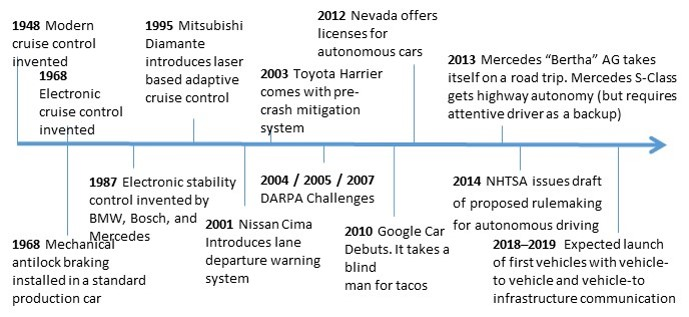
\includegraphics{image/Historical development of autonomous driving.jpeg}
    \caption{The historical development of autonomous driving~\cite{inbook}.}
    \label{fig:historical_development}
\end{figure}

In today's world, developing and using software has become very important across many industries. While these software solutions provide us with numerous conveniences and advantages, they also introduce certain requirements. One of the most critical requirements for any software is testing. The testing phase can be used to determine whether an application fulfills its intended function or to assess its efficiency. Of course, in some sectors, this functionality takes on an even greater importance. One such area is safety. In industries like aviation and automotive, where a user's safety can be directly affected by an error in the application, testing and simulation are more important than ever. In model-based software applications, after a model is created, it moves to the verification stage. Before being loaded onto the hardware, the model undergoes several verification steps (as the V-model in Figure~\ref{fig:v_model}). Some of these verifications are named \ac{MIL}~\cite{plummer-2006}, \ac{SIL}~\cite{4455268}, and \ac{HIL}~\cite{fathy-2006}.

\textbf{\acs{MIL}} In the initial stages of system design, before real hardware or software components are implemented, the simulation and testing of system models are carried out by the \ac{MIL} testing method. This method uses mathematical models and simulations for system or component design. These models are utilized to understand how the designed system will function and behave. \ac{MIL} testing is a critical tool for verifying the design and identifying potential problems at an early stage. With this method, engineers and designers can gain valuable insights into how the system will operate before actually manufacturing the hardware or fully developing the software.

\textbf{\acs{SIL}} The \ac{SIL} testing method is the process of testing a system or component's software without using real hardware. This method simulates environmental factors or other parts interacting with the system while the software runs directly on a computer. This simulation evaluates the software's behavior and performance under real-world conditions. The main goal of \ac{SIL} testing is to verify the software's functionality, detect errors at an early stage, and analyze interactions between the system and the software. This approach accelerates the software development and refinement processes and prevents costly errors.

\textbf{\acs{HIL}} The \ac{HIL} testing method creates an environment to control and test real hardware. In this method, the hardware being tested, such as a vehicle control unit, operates in real time, but the software simulates the physical systems (e.g., engines, sensors, actuators, etc.) interacting with the hardware in real time. This simulation allows for the evaluation of how the hardware performs under real-world conditions.

\begin{figure}[htbp]
    \centering
    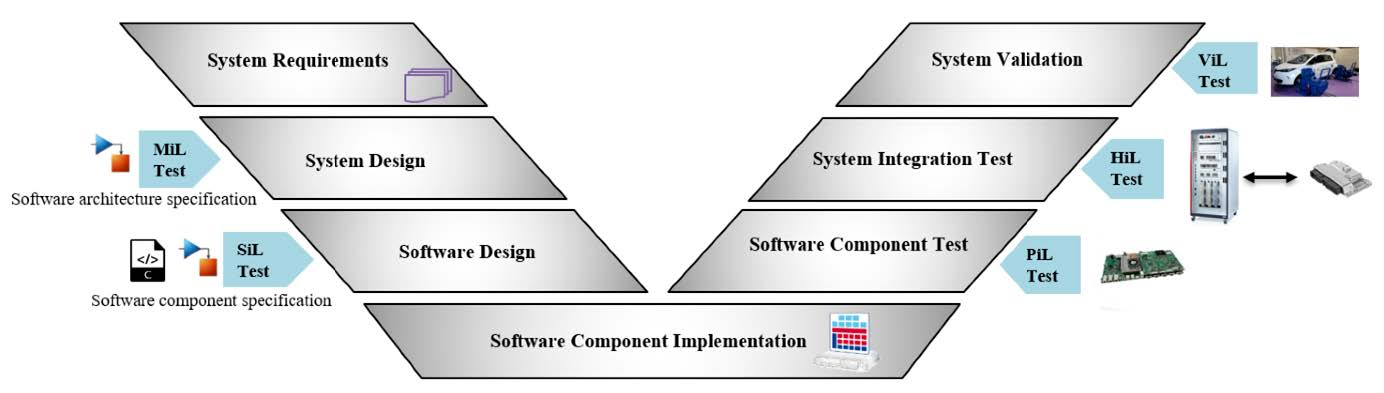
\includegraphics{image/v cycle development process.jpeg}
    \caption{\acs{MIL}, \acs{SIL}, PIL, \acs{HIL} and \acs{VIL} tests in the V-cycle development process~\cite{article}.}
    \label{fig:v_model}
\end{figure}

In Figure~\ref{fig:driving_test_simulator} a driving test simulator is shown. Test simulators typically fall under the \ac{SIL} category. The \ac{SIL} testing method has numerous advantages. These benefits explain why \ac{SIL} tests are an important part of the software development process and demonstrate their value to engineers and developers across various industries. The main advantages can be listed as follows:

\textbf{Cost Efficiency:} \ac{SIL} tests are conducted in a simulated environment that does not require real hardware, thus reducing the costs associated with purchasing, maintaining, and repairing hardware. Additionally, early diagnosis of potential errors helps prevent more costly problems later on.

\textbf{Rapid Feedback Loop:} Testing software in a model allows for quick iterations in the development process. This enables developers to instantly see the effects of their code and make fast modifications if necessary.

\textbf{Risk Reduction:} Tests conducted without real hardware use a simulated environment to safely examine situations that could be potentially dangerous or harmful to the hardware. This is especially important when expensive hardware is involved.

\textbf{Broad Test Scenarios:} \ac{SIL} tests are capable of quickly and easily testing a wide range of scenarios that mimic real-world conditions. Developers can experiment with system parameters, error states, and various operational conditions.

\textbf{Acceleration of the Development Process:} \ac{SIL} tests can speed up the development process instead of waiting for the hardware to be ready. Testing the software alongside hardware development shortens the time to market for the product.

\textbf{Preparation for Integration and System Tests:} When software is successfully tested in a \ac{SIL} environment, the transition to more complex testing stages where hardware and software are run together becomes easier. This helps reduce problems that may arise during system tests and integration.

\begin{figure}[htbp]
    \centering
    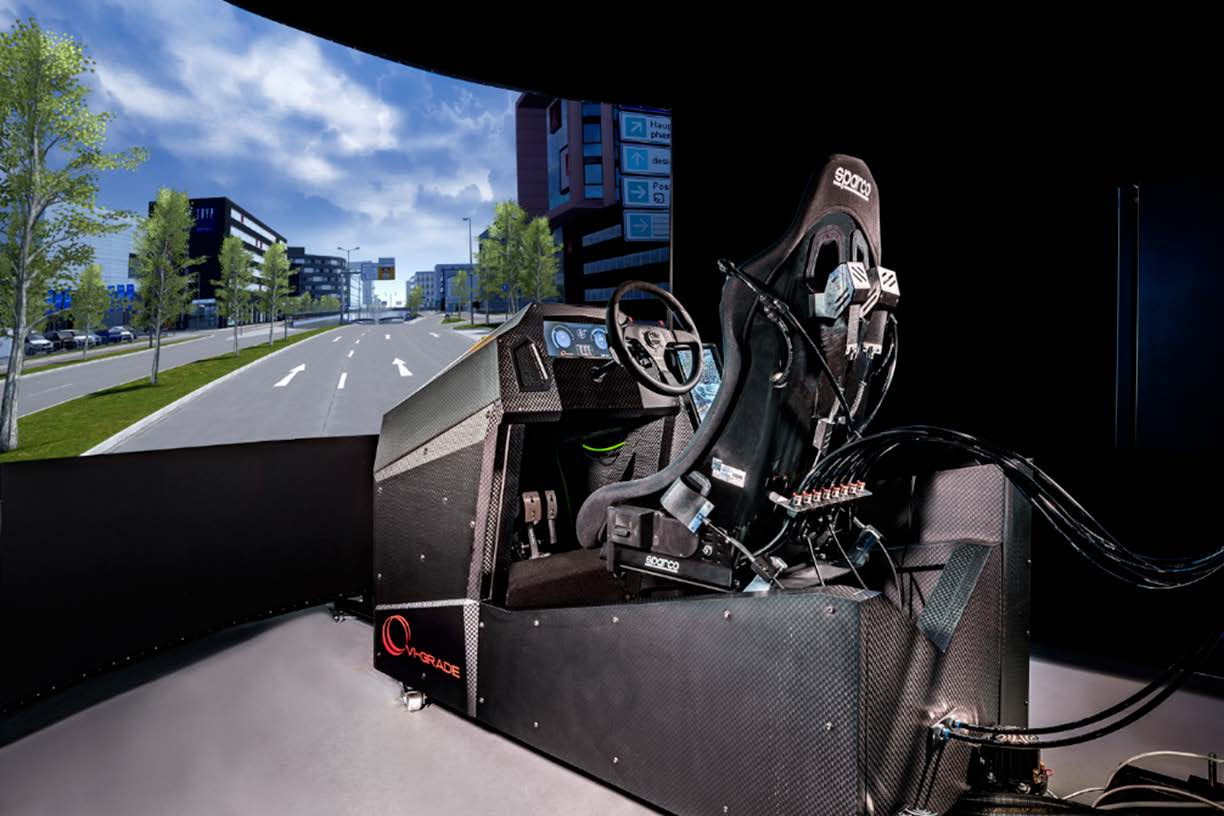
\includegraphics{image/driving test simulator.jpeg}
    \caption{Driving test simulator~\cite{Sim}.}
    \label{fig:driving_test_simulator}
\end{figure}

\textbf{Flexibility in the Development Process:} Software can be tested and developed with various hardware platforms and configurations. This flexibility allows for the evaluation of how the software will perform on different systems.

\section{State of the Art in Autonomous Driving Simulators}
Advancements in the field of autonomous driving have also led to the development of powerful autonomous driving simulators. Nowadays, a wide range of simulators produced by various companies are in use. These include open-source projects (e.g.\ CARLA~\cite{dosovitskiy-2017}, AirSim~\cite{shah-2017}), commercial software, and customized simulation solutions used in academic and industrial research. In the context of this thesis, a simulation environment is essential, because the \acf{LKA} function is developed and evaluated entirely in a virtual \ac{VIL} setup rather than on a physical test vehicle. Therefore, it is crucial to clearly define the requirements that the simulator must satisfy---such as realistic sensor models, controllable traffic and weather, and reproducible scenarios---and to justify the choice of a specific platform.

In the following, I first review several popular autonomous driving simulation tools and platforms available in the literature and in practice. The comparison focuses on criteria such as graphic quality, accuracy of the physics engine, sensor simulation capabilities, simulation of traffic and pedestrians, weather conditions, and the ability to simulate at different times of the day. Based on these criteria, I motivate the selection of CARLA as the main simulation platform for this work and explain how it will be used to implement and test the proposed \ac{LKA} function.

\subsection{Waymo simulator}
\begin{figure}[htbp]
    \centering
    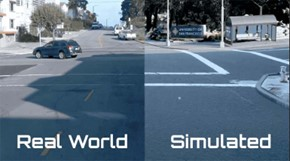
\includegraphics{image/waymo real world comparison.jpeg}
    \caption{Comparing Waymo Simulator graphics and the real world.}
    \label{fig:waymo}
\end{figure}
Waymo possesses an advanced simulation platform~\cite{gulino2023waymaxaccelerateddatadrivensimulator} and is widely recognized as a leader in \ac{AV} technology. This simulator plays a crucial role in the development and testing of autonomous driving systems by providing a highly realistic (as can be seen in Figure~\ref{fig:waymo}) and comprehensive virtual environment. It combines high-fidelity graphics that accurately replicate real-world environments with a precise physics engine capable of modeling vehicle dynamics, collisions, and surface interactions. Furthermore, it includes detailed sensor emulation for LIDAR, radar, and cameras, enabling a realistic representation of environmental perception. The platform can also model complex traffic flow and pedestrian behaviors, which are essential for evaluating \acsp{AV} in dense urban settings. In addition, the simulator supports a wide range of weather and lighting conditions, allowing performance assessment under rain, snow, fog, or low-light scenarios. Owing to these capabilities, the Waymo simulator holds a significant position among state-of-the-art autonomous driving simulation platforms.

\subsection{SVL Simulator}
\begin{figure}[htbp]
    \centering
    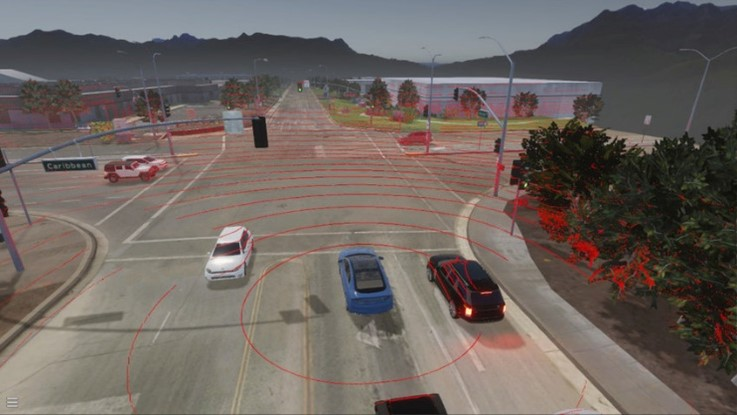
\includegraphics{image/svl screen.jpeg}
    \caption{SVL Simulator Screen.}
    \label{fig:svl}
\end{figure}
The \ac{AV} research community frequently employs the LGSVL Simulator~\cite{rong2020lgsvlsimulatorhighfidelity}, an open-source platform designed for high-fidelity testing of perception and control algorithms. Thanks to its Unity-based rendering engine, LGSVL offers realistic visual environments suitable for evaluating camera-based functions. Its physics engine provides detailed modeling of vehicle dynamics, tire--road interactions, and collisions, enabling credible closed-loop testing of control algorithms. The simulator includes configurable sensor models---such as lidar, radar, and cameras---along with comprehensive traffic and pedestrian behavior, allowing researchers to model complex urban scenarios (Figure~\ref{fig:svl}). Furthermore, LGSVL supports diverse weather and lighting conditions, which makes it valuable for assessing the robustness of autonomous driving functions under varying environmental circumstances. LGSVL represents an important reference point when comparing available simulation platforms.

\subsection{Sim4CV}
\begin{figure}[htbp]
    \centering
    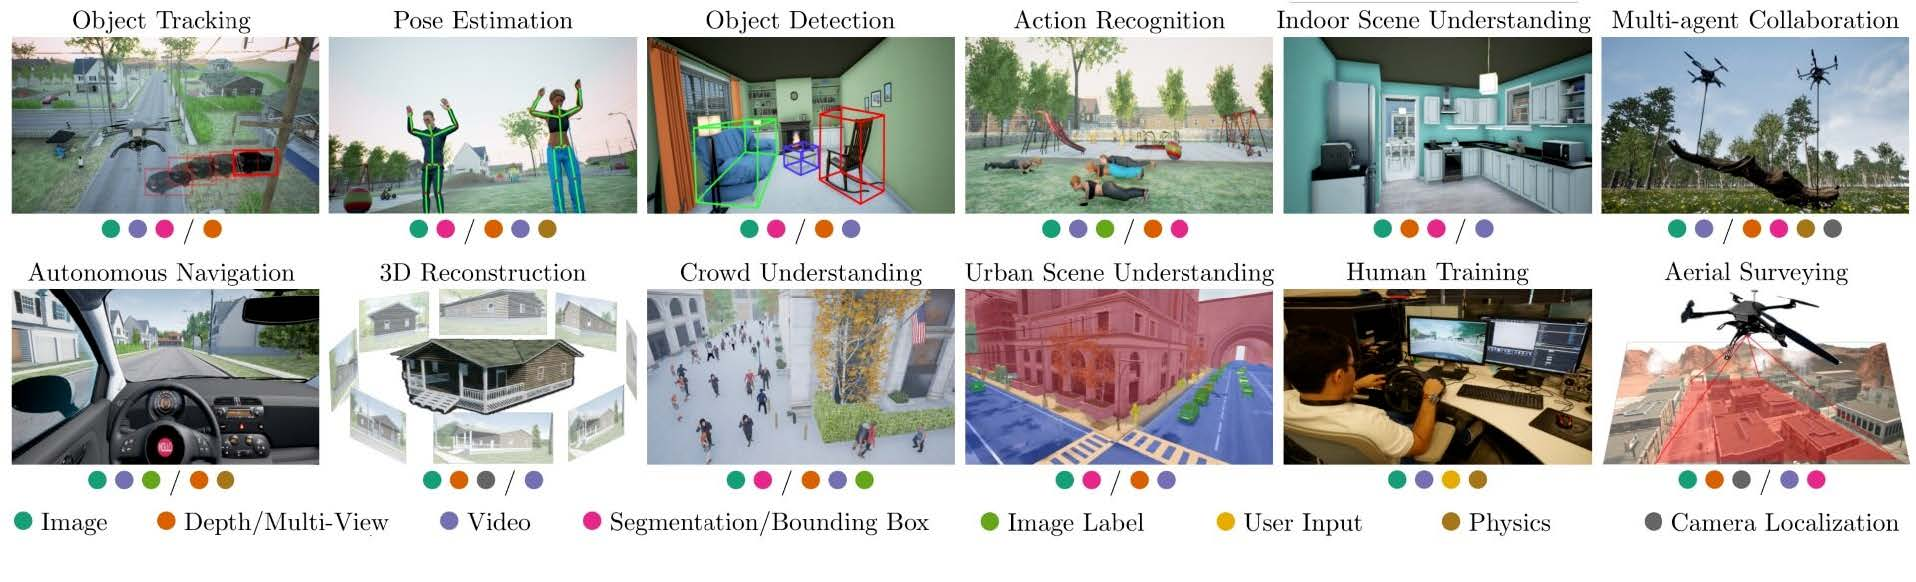
\includegraphics{image/sim4cv.jpeg}
    \caption{Sim4CV: A Photo-Realistic Simulator for Computer Vision Applications.}
    \label{fig:sim4sv}
\end{figure}
Sim4CV is a simulation platform developed for research in computer vision and autonomous systems, with a strong emphasis on autonomous driving and aerial navigation~\cite{muller-no-date}. Built on Unreal Engine 4, it provides high-quality visual environments and a physics engine capable of modeling realistic vehicle dynamics, object interactions, and environmental effects. The platform supports the simulation of various sensors, including cameras and lidar, enabling detailed testing of perception algorithms. Sim4CV also offers traffic and pedestrian simulation, though the level of sophistication may vary across versions and configurations (Figure~\ref{fig:sim4sv}). Furthermore, the ability to adjust weather and lighting conditions makes it suitable for evaluating algorithm robustness under diverse environmental scenarios.

\subsection{CARLA Simulator}
\begin{figure}[htbp]
    \centering
    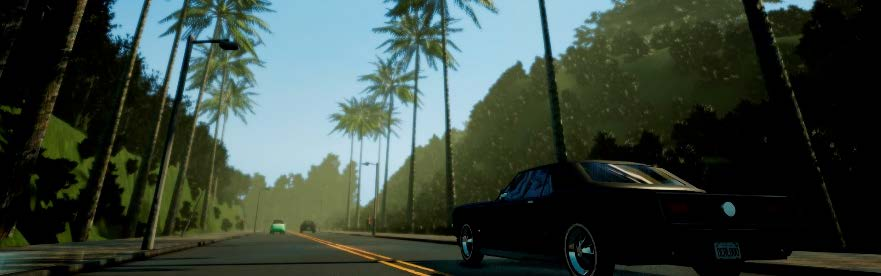
\includegraphics{image/carla screen2.jpeg}
    \caption{CARLA Simulator Screen.}
    \label{fig:carla_screen}
\end{figure}
The CARLA Simulator is an open-source autonomous driving platform~\cite{team-no-date} widely used in research for developing, testing, and validating \ac{AV} algorithms. Built on Unreal Engine 4, it provides high-fidelity graphics that closely resemble real-world environments (Figure~\ref{fig:carla_screen}), which is essential for evaluating perception systems. The underlying physics engine of CARLA accurately models vehicle dynamics, collisions, and surface interactions, enabling realistic assessment of control and planning algorithms. It also offers comprehensive sensor simulation---including cameras, LIDAR, radar, and GNSS---allowing researchers to replicate and analyze diverse sensing conditions. In addition, CARLA supports dynamic traffic scenarios and human-like pedestrian behavior, creating complex and socially interactive environments for autonomous driving studies. Finally, its configurable weather and lighting system makes it possible to test algorithms across various environmental conditions, ensuring robustness and generalizability in real-world deployments.

\begin{table}[htbp]
    \centering
    \footnotesize
    \begin{tabular}{@{}p{4.6cm}cccc@{}}
        \hline
        Features / Simulators & Waymo & LGSVL & Sim4CV & CARLA \\
        \hline
        Graphics Quality                     & 8/10 & 9/10 & 8/10 & 9/10 \\
        Physics Engine Accuracy              & 8/10 & 9/10 & 7/10 & 9/10 \\
        Sensor Simulation                    & 8/10 & 9/10 & 7/10 & 9/10 \\
        Traffic and Pedestrian Simulation    & 8/10 & 9/10 & 6/10 & 9/10 \\
        Weather Conditions                   & 7/10 & 8/10 & 6/10 & 9/10 \\
        Simulation at Different Times of Day & 7/10 & 8/10 & 6/10 & 9/10 \\
        \hline
    \end{tabular}
    \caption{Comparative Feature Scoring of Simulators.}
    \label{tab:simulators}
\end{table}
Using a set of predefined evaluation criteria---such as graphics quality, physics realism, sensor simulation, traffic modeling, and environmental variability---a comparative score was assigned to each simulator. Table~\ref{tab:simulators} summarizes the evaluation results based on these criteria.

\section{ADAS Applications}
\ac{ADAS} are becoming increasingly common in today's vehicles. Developed to enhance vehicle safety and the driving experience, these systems utilize various technologies such as cameras, sensors, and radars to identify potential hazards and are designed to alert the driver or automatically control the vehicle under certain conditions. \acs{ADAS} technologies not only assist drivers in traveling more safely and comfortably but also have the potential to reduce traffic accidents. There are various applications of \acs{ADAS}, which are crucial for the safety of the driver and also provide significant conveniences. Some of these applications can be briefly discussed as follows:

\begin{wrapfigure}{r}{0pt}
    \centering
    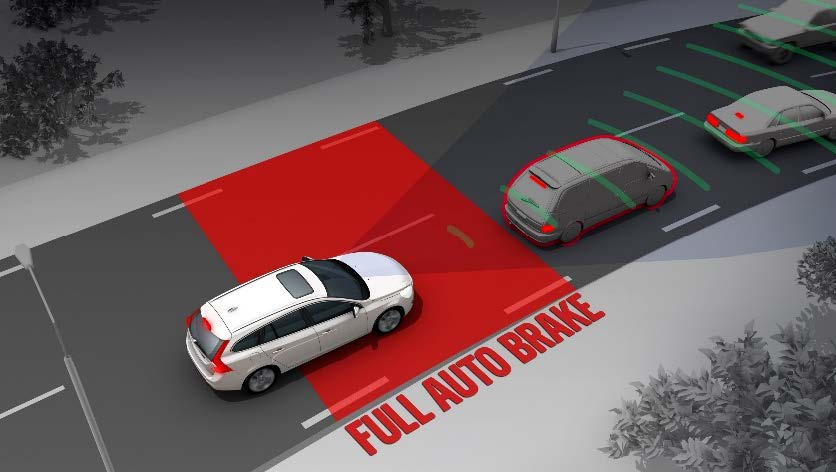
\includegraphics{image/emergency braking.jpeg}
    \caption{Automatic Emergency Braking system.}
    \label{fig:emergency_breaking}
\end{wrapfigure}

\textbf{Automatic Emergency Braking:} The vehicle automatically brakes to avoid colliding with a vehicle or obstacles ahead~\cite{5625077}. A laser radar sensor detects the distance to the vehicle ahead and the relative speed. If there is an object in the area seen by the laser radar sensor at this speed, the brakes are activated to prevent a collision as shown in Figure~\ref{fig:emergency_breaking}. Additionally, in some vehicles, it works in conjunction with seat belts activated by braking before a collision to help reduce injuries in cases where a collision is unavoidable.

\begin{wrapfigure}{l}{0pt}
    \centering
    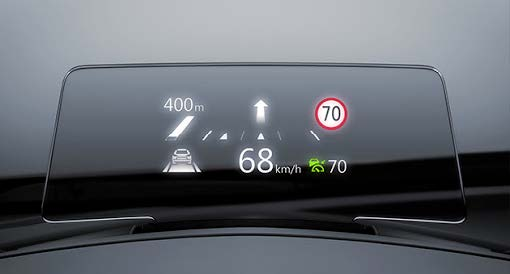
\includegraphics{image/traffic sign.jpeg}
    \caption{Traffic Sign Recognition System.}
    \label{fig:traffic}
\end{wrapfigure}

\textbf{Traffic Sign Recognition System:} This system detects traffic signs and informs the driver about traffic rules such as speed limits and prohibition signs. Generally, an image is captured by a camera sensor placed on the vehicle's windshield, and the detected image is projected onto the user's screen (Figure~\ref{fig:traffic}). This technology aims to prevent accidents by ensuring that drivers do not overlook important warning signs on the road~\cite{fu-2010}.

\begin{wrapfigure}{r}{0pt}
    \centering
    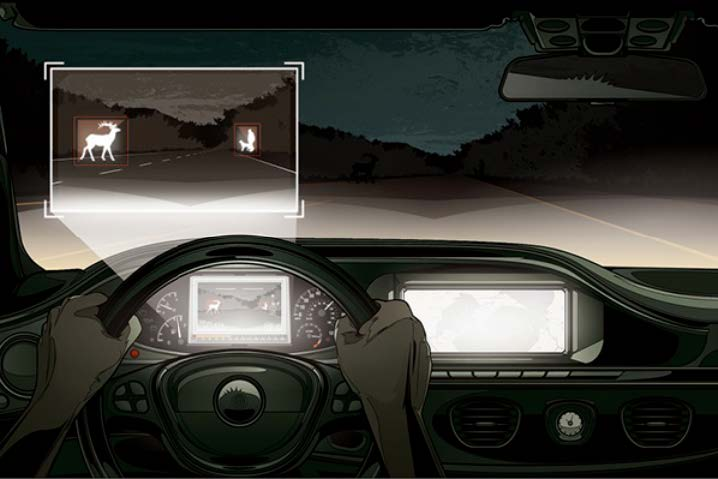
\includegraphics{image/night vision.jpeg}
    \caption{Night Vision.}
    \label{fig:Night}
\end{wrapfigure}

\textbf{Night Vision:} This system expands the driver's field of vision in low-light conditions or at night through cameras or other sensors~\cite{kupper-2002}. Utilizing thermal cameras and infrared lights, it detects living beings on the road ahead and provides audible or visual warnings to the driver (Figure~\ref{fig:Night}). In addition to detection, advanced night vision systems can highlight potential hazards directly on the dashboard display or head-up display.

\begin{wrapfigure}{l}{0pt}
    \centering
    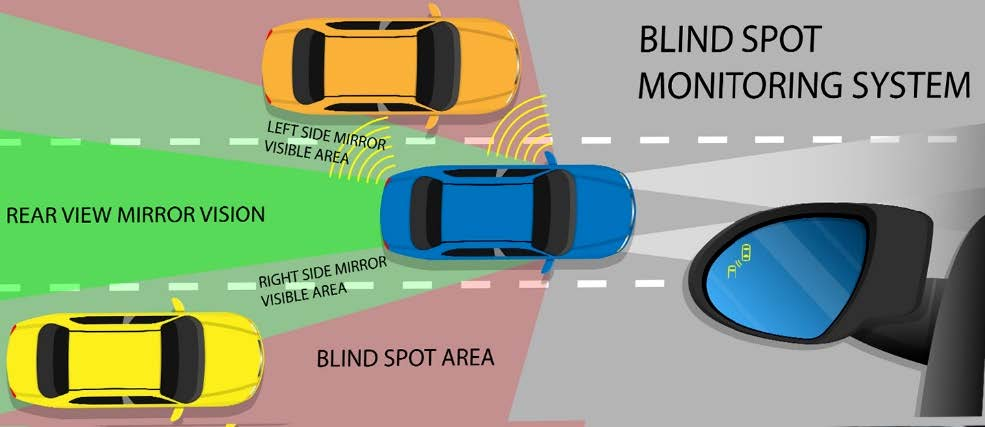
\includegraphics[width=0.5\textwidth]{image/blind spot.jpeg}
    \caption{Blind Spot Warning System.}
    \label{fig:blind_spot}
\end{wrapfigure}

\textbf{Fatigue Detection Systems:} Various studies have suggested that approximately 20\% of all road accidents, and up to 50\% on certain roads, are fatigue-related~\cite{wikipedia-contributors-2025}. Although the implementation of this system varies among manufacturers, some brands warn the driver by detecting steering movements and how often the vehicle drifts out of its lane.

\textbf{Blind Spot Warning System:} This system identifies the presence of other vehicles in the vehicle's blind spots and informs the driver about them. Vehicles in the blind spot are detected using radar sensors located on the sides of the rear bumper (Figure~\ref{fig:blind_spot}). A warning is displayed to the driver in the side mirror, and if the driver signals to change lanes while there is a vehicle in the blind spot, an alert is issued. In some models, changing lanes by braking is prevented to enhance the safety of the driver in the car and to avoid road accidents~\cite{liu-2017}.

\begin{wrapfigure}[11]{r}{0pt}
    \centering
    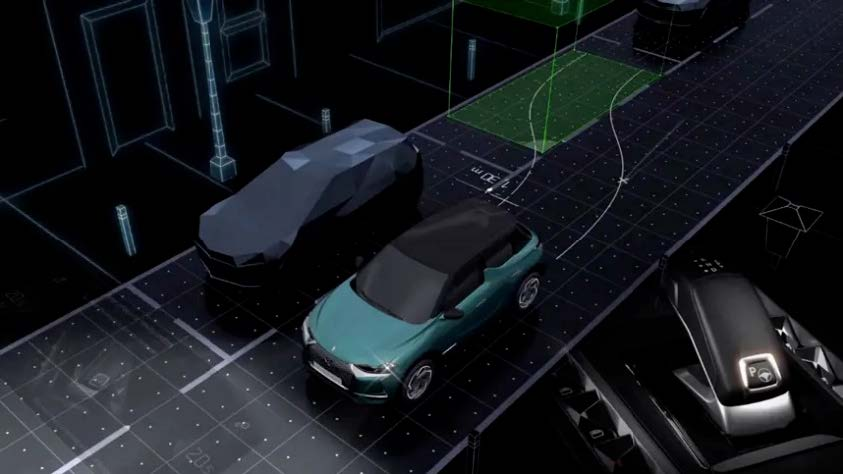
\includegraphics{image/parking assistant.jpeg}
    \caption{Parking Assistant.}
    \label{fig:parking_assist}
\end{wrapfigure}

\textbf{Parking Assistant:} This feature assists the driver in better positioning the vehicle while parking and, in some cases, can automatically park the vehicle (Figure~\ref{fig:parking_assist}). It utilizes parking sensors located around the vehicle to do this~\cite{7548171}. Parking sensors are generally electromagnetic sensors. Commonly, the system is used in a manner where the driver is still responsible for commands such as gas and gear changes.

\begin{wrapfigure}{l}{0pt}
    \centering
    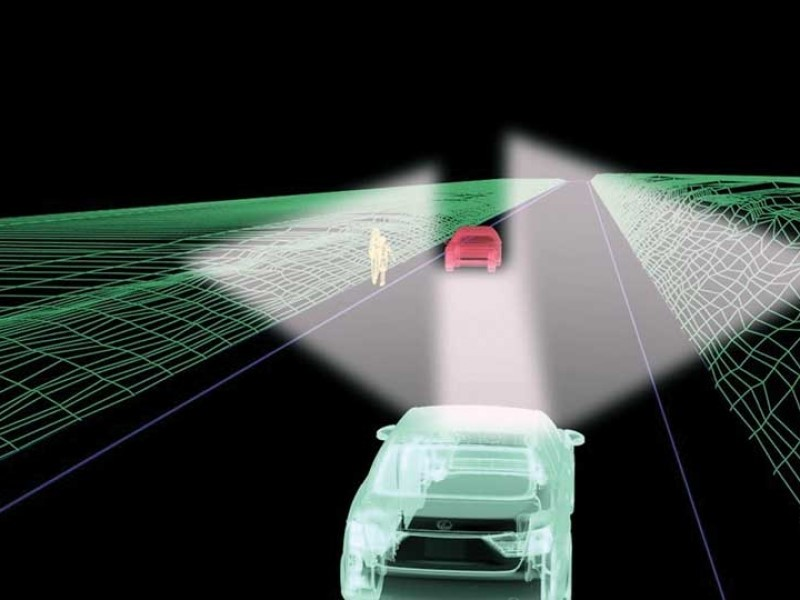
\includegraphics{image/automatic headlight control.jpeg}
    \caption{Automatic Headlight Control.}
    \label{fig:automatic_headlight}
\end{wrapfigure}

\textbf{Automatic Headlight Control:} The effectiveness of vehicle headlights becomes even more crucial on roads with insufficient external lighting at night, such as forest roads. Oncoming drivers on these types of roads can be affected by the headlight beams. Systems like this reduce the light intensity when detecting an oncoming vehicle to minimize the adverse effects on the opposite driver. In more advanced models, the direction of the headlight beam is adjusted to achieve this effect (Figure~\ref{fig:automatic_headlight}).

\begin{wrapfigure}{r}{0pt}
    \centering
    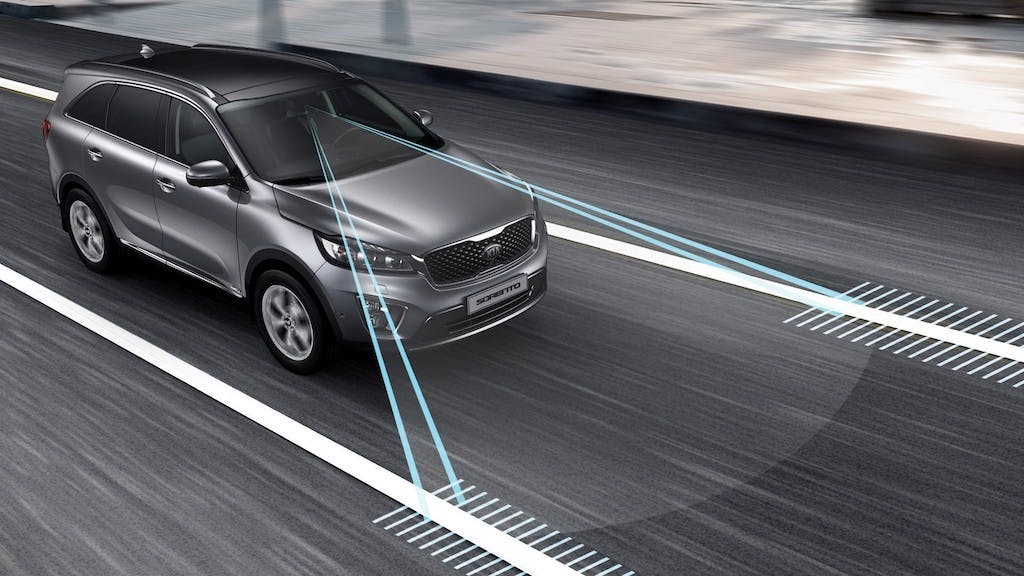
\includegraphics{image/lane keeping.jpeg}
    \caption{\acs{LKA} demonstration.}
    \label{fig:lane_keeping_assist}
\end{wrapfigure}

\textbf{\acl{LKA}:} This system uses a camera sensor to detect the distance of the vehicle from the lane markings and activates when the determined distance falls below a certain threshold (Figure~\ref{fig:lane_keeping_assist}). It steers the steering wheel to direct the vehicle back into the lane, ensuring it remains within its lane boundaries. It acts as a countermeasure to unintentional drifting, reducing relevant accidents by over 20\%.

\begin{wrapfigure}{l}{0pt}
    \centering
    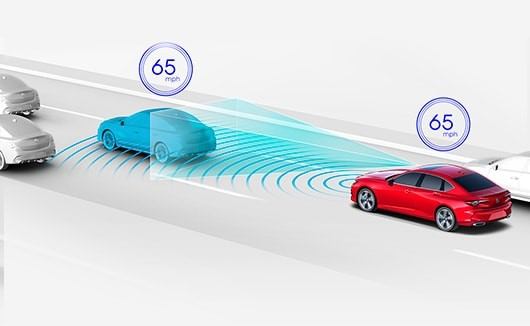
\includegraphics{image/acc.jpeg}
    \caption{Adaptive Cruise Control.}
    \label{fig:adaptive_cruise}
\end{wrapfigure}

\textbf{Adaptive Cruise Control:} This system is a more advanced version of the traditional cruise control system~\cite{my-car-does-what-2018}. While traditional cruise control maintains the vehicle at a set speed, this system adapts the speed based on the speed of the vehicle ahead (Figure~\ref{fig:adaptive_cruise}). It utilizes two separate sensors to accomplish this. The first sensor is a radar sensor that measures the distance to the vehicle in front. The second sensor is a speed sensor that detects any decrease or increase in the vehicle's speed. Based on the information from these sensors, decisions are made and implemented to accelerate or decelerate. Generally, the desired distance and following speed can be adjusted by the user via controls on the steering wheel.

\section{Related Works}
The research community has proposed various methods for validating autonomous driving functions using simulation and \ac{VIL} concepts, as well as a wide range of lateral control strategies for path and lane tracking. This section summarizes the most relevant works and explains how they relate to the present thesis, which implements a \ac{LKA} function in the CARLA simulator using an external Python-based controller and an RGB camera.

\paragraph{\acs{VIL} simulation}
Son et al.\ propose a PG-based \ac{VIL} simulation framework that combines a real vehicle with a virtual driving environment for system development and consistency validation~\cite{electronics11244073}. Their system includes modules for virtual road generation, synchronization between real and virtual domains, a virtual traffic manager, and perception sensor modelling. They demonstrate that the behavior observed in the \ac{VIL} simulation setup is consistent with physical vehicle tests over different speeds, road types, and surrounding environments. This work shows how \ac{VIL} can improve reproducibility and safety when testing autonomous driving systems.

Cheng et al.\ provide a comprehensive survey on testbench-based Vehicle-in-the-Loop simulation testing for \acsp{AV}~\cite{survey_test_bench}. They review existing \ac{AV} testing approaches and identify limitations of traditional methods. The paper then focuses on testbench-based \ac{VIL} architectures, principles, and equipment, with particular emphasis on physical signal stimulation and realistic road condition simulation. The survey identifies research gaps between current testbench technologies and industrial \ac{AV} testing needs, and highlights \ac{VIL} as a promising tool for accurate and efficient validation.

Xiong Hu et al.\ present a \ac{VIL} simulation test framework for \acsp{AV}, where an autonomous driving system is evaluated using a virtual environment combined with real vehicle components~\cite{xiong_hu}. Their work emphasizes the synchronization of vehicle dynamics and simulated scenarios and discusses how \ac{VIL} can be used to test autonomous driving functions safely and systematically.

These works clearly show that \ac{VIL} is an important methodology for validating autonomous driving systems. However, they mainly focus on general architectures, testbench setups, and system-level validation. They do not specifically address a software-only \ac{VIL} configuration in a driving simulator like CARLA, where a simulated vehicle is controlled by external code using RGB camera images. Furthermore, the detailed design and evaluation of a single \acs{ADAS} function such as \ac{LKA}---implemented and tested entirely in such a \ac{VIL} setup---remains less explored. This is where the present thesis contributes.

\paragraph{Lateral control for \acsp{AV}}
Lateral control is a key component for lane keeping and path tracking. Kebbati et al.\ provide a technical review of lateral control methods for autonomous wheeled vehicles~\cite{kebbati}. They classify control approaches into model-based and data-driven methods, and discuss their advantages, limitations, and implementation challenges. The survey underlines that lateral control must deal with accuracy, robustness, and real-time constraints, and highlights open challenges for future research.

Artu\~{n}edo et al.\ present a comparative evaluation of state-of-the-art lateral control strategies for \acsp{AV}~\cite{ARTUNEDO2024100910}. They propose a systematic tuning methodology and define a comprehensive set of performance metrics covering tracking accuracy, robustness, and comfort. The controllers are evaluated in extensive simulations and real-vehicle tests over different trajectories and scenarios. Their results show how different control strategies behave under the same conditions and provide guidance for selecting suitable lateral controllers.

Dominguez et al.\ experimentally compare several classical lateral controllers---such as Pure Pursuit and Stanley---on an \ac{AV} platform~\cite{7795743}. They study the performance of these controllers in terms of tracking error and stability, using a combination of simulation and real-world experiments. Their work provides practical insight into the behavior of commonly used path-tracking controllers and their suitability for autonomous driving applications.

Snider's technical report is a widely cited reference on automatic steering methods for autonomous automobile path tracking~\cite{Snider2009AutomaticSM}. It describes the mathematical formulation and implementation details of several steering controllers, including Pure Pursuit and Stanley, and discusses their application to \acsp{AV}. This report is frequently used as a theoretical foundation when implementing classical lateral control laws.

These studies provide a solid theoretical and experimental basis for the lateral control part of \ac{LKA}. However, most of them either assume ideal path or lane information (for example, predefined waypoints or ground-truth lane geometry) or focus on real-vehicle experiments without an explicit simulation-based \ac{VIL} framework. They do not analyze in detail how classical lateral controllers perform when they receive lane information from a real-time camera-based perception pipeline inside a simulator.

\paragraph{Identified gap and relation to this thesis}
In summary, the literature on \ac{VIL} shows how combined real--virtual setups can be used to validate autonomous driving systems~\cite{electronics11244073, survey_test_bench, xiong_hu}, while the lateral control literature provides a variety of controllers and comparative evaluations for path and lane tracking~\cite{kebbati, ARTUNEDO2024100910, 7795743, Snider2009AutomaticSM}. However, the combination of these two aspects,
\begin{itemize}
    \item a \textbf{\acs{VIL}-style simulation environment} in a high-fidelity simulator, and
    \item a \textbf{camera-based \acs{LKA} function} implemented as an external control stack,
\end{itemize}
is less represented in the existing works.

The present thesis addresses this gap by implementing a modular \ac{LKA} system in CARLA, where an RGB camera provides input to an external Python program that estimates lane geometry and computes steering commands. The system is evaluated in a reproducible simulation environment, thus connecting the ideas of \ac{VIL}-based validation and classical lateral control within a single, integrated \ac{LKA} framework.

% chapters/chapter2.tex  — converted from chapter2.typ
% Conventions used (identical to chapter1.tex):
%   Typst @KEY            -> \ac{KEY}        (auto: long on first use, short after)
%   Typst @KEY:pls        -> \acsp{KEY}      (short plural, e.g. "AVs")
%   Typst @figlabel       -> Figure~\ref{fig:figlabel}
%   Typst @citekey        -> \cite{citekey}
%   Typst @ch3[Chapter]   -> Chapter~\ref{ch3}
%   Typst @app:b          -> Appendix~\ref{app:b}
% Inside captions \acs{} is used so float placement cannot disturb first-use timing.
%
% NOTE: \ref{ch3} and \ref{app:b} need matching \label{ch3} (chapter3.tex) and
%       \label{app:b} (the appendix in main.tex) to resolve. Add them if missing.

\chapter{Interface Co-Simulation Design}
\label{ch2}

\section{Selecting the Suitable Simulator}
The development and testing of autonomous driving technologies require a robust simulation environment. This environment must accurately model the real world, including vehicles, pedestrians, and various environmental conditions, while also providing comprehensive support for sensor simulation and enabling integration with analytical tools. After a detailed evaluation of existing simulators, including the Waymo Simulator, LGSVL Simulator, Sim4CV, and CARLA Simulator, based on critical features such as graphic quality, the accuracy of the physics engine, sensor simulation capabilities, the simulation of traffic and pedestrians, weather conditions, the ability to simulate different times of day, CARLA Simulator has been identified as the most suitable choice for my research objectives. CARLA provides high-quality graphics with Unreal Engine 4~\cite{unreal_engine_4} and its physics engine accurately models vehicle dynamics and environmental interactions, offering a solid foundation for testing autonomous driving algorithms under various conditions. Moreover, its ability to simulate a wide range of sensors used in \acsp{AV}, such as cameras, LIDAR, radar, and GNSS, with high fidelity is crucial for the development and testing of perception algorithms. CARLA also excels in simulating dynamic traffic scenarios and pedestrian behaviors, facilitating comprehensive testing of autonomous driving systems in complex urban environments. The capability to simulate different weather conditions and times of day is important for assessing the performance of \ac{AV} systems under various environmental conditions. For my research, Python API of CARLA facilitates easy integration with an external controller, providing a seamless workflow for data analysis and algorithm testing. Consequently, CARLA Simulator's advanced graphics, accurate physics engine, extensive sensor simulation capabilities, and effective traffic and pedestrian simulation set it as the ideal choice for my autonomous driving research. Its compatibility with Python API further supports my analytical and development needs, making it the most suitable simulator for my project.

\section{Modeling the Car in the Environment}
In order to control a vehicle in the simulation, the controller must recognize the vehicle model. For this, a model of the vehicle is needed. Various models can be used when modeling the vehicle. Among these, the most commonly used ones usually offer a good balance between simplicity and accuracy, capable of representing the vehicle's motion dynamics and control systems. In line with the needs of this project, the \ac{DST} model has been chosen (shown in Figure~\ref{fig:single_track}). The \acs{DST} model (bicycle model) can be modeled with single-track wheels (one front and one rear wheel). This is equivalent to a model where the right and left sides of a four-wheeled vehicle are considered equal.

\begin{figure}[htbp]
    \centering
    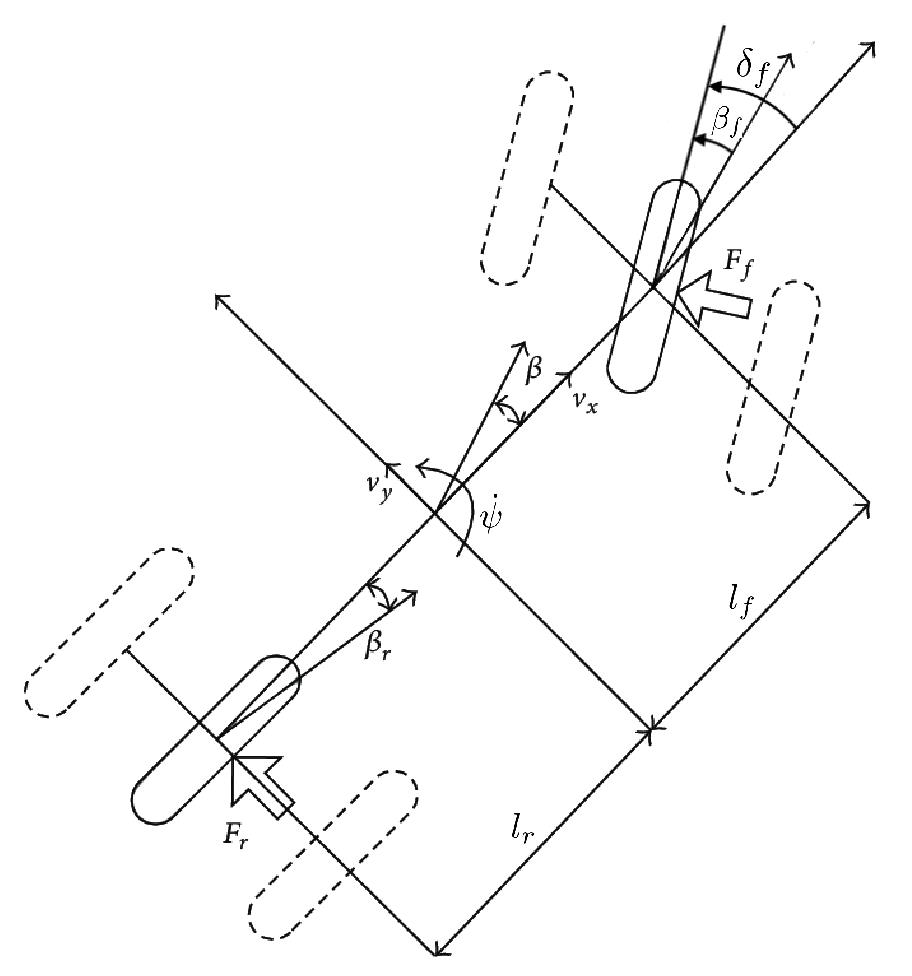
\includegraphics{image/single track model.jpeg}
    \caption{Single Track Model.}
    \label{fig:single_track}
\end{figure}

\noindent\textbf{Vehicle variables:}
\begin{itemize}
    \item $\delta_f$: steering angle.
    \item $\beta$: vehicle sleep angle $=$ angle between the vehicle longitudinal axis and velocity.
    \item $\beta_f, \beta_r$: tire slip angles $=$ angles between the tire longitudinal axis and velocity.
\end{itemize}

\noindent\textbf{Vehicle parameters:}
\begin{itemize}
    \item \acs{CoG}: center of gravity
    \item $m, J$: mass and moment of inertia
    \item $l_f$: distance \acs{CoG} -- front wheel center
    \item $l_r$: distance \acs{CoG} -- rear wheel center
    \item $c_f, c_r$: front/rear cornering stiffnesses.
\end{itemize}

\begin{figure}[htbp]
    \centering
    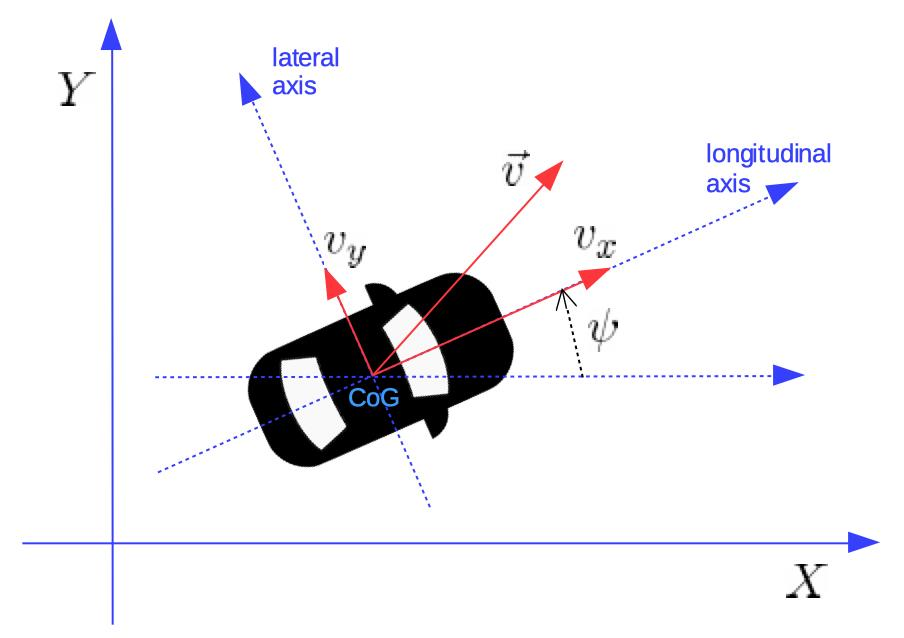
\includegraphics{image/vehicle reference system.jpeg}
    \caption{Vehicle Reference System.}
    \label{fig:Vehicle_reference}
\end{figure}

\noindent\textbf{Vehicle Dynamic parameters:}
\begin{itemize}
    \item $X, Y$: coordinates of the vehicle \acs{CoG} in an inertial reference frame (shown in Figure~\ref{fig:Vehicle_reference})
    \item $\psi$: yaw angle
    \item $\omega_\psi = \dot{\psi}$: yaw rate
    \item $\vec{v} \equiv V$: velocity vector in the inertial frame
    \item $v_x$: longitudinal speed $= \vec{v}$ component along the longitudinal axis
    \item $v_y$: lateral speed $= \vec{v}$ component along the lateral (transverse) axis
    \item $a_x$: longitudinal acceleration in the inertial frame.
\end{itemize}

The state equations of the \acs{DST} model are:
\begin{align}
    \dot{X}           &= V_x \cos\psi - V_y \sin\psi \\
    \dot{Y}           &= V_x \sin\psi + V_y \cos\psi \\
    \dot{\psi}        &= \omega_\psi \\
    \dot{V}_x         &= V_y \omega_\psi + a_x \\
    \dot{V}_y         &= -V_x \omega_\psi + \frac{2}{m}\left(F_{yf} + F_{yr}\right) \\
    \dot{\omega}_\psi &= \frac{2}{J}\left(l_f F_{yf} - l_r F_{yr}\right)
\end{align}

where $F_{yf}$ and $F_{yr}$ are the lateral forces exchanged between tire and road.

For the tire model, there are several tire model options:

\medskip
\noindent\textbf{Linear (for $V_x = \mathrm{const}$) tire model:}
\begin{equation}
    F_{yf} = -C_f \beta_f, \hspace{1.5em} F_{yr} = -C_r \beta_r
\end{equation}
\begin{equation}
    \beta_f = \frac{V_y + l_f \omega_\psi}{V_x} - \delta_f, \hspace{1.5em} \beta_r = \frac{V_y - l_r \omega_\psi}{V_x}
\end{equation}

\noindent\textbf{Nonlinear simplified tire model:}
\begin{equation}
    F_{yf} = -C_f \beta_f \cos\delta_f, \hspace{1.5em} F_{yr} = -C_r \beta_r
\end{equation}
\begin{equation}
    \beta_f = \arctan\!\left(\frac{V_y + l_f \omega_\psi}{V_x}\right) - \delta_f, \hspace{1.5em} \beta_r = \arctan\!\left(\frac{V_y - l_r \omega_\psi}{V_x}\right)
\end{equation}

\noindent\textbf{Nonlinear Pacejka tire model:}
\begin{equation}
    F_{yf} = -f_p(\beta_f)\cos\delta_f, \hspace{1.5em} F_{yr} = -f_p(\beta_r)
\end{equation}
where $\beta_f$ and $\beta_r$ and $f_p(\beta)$ is given by the Pacejka magic formula.

\noindent\textbf{Pacejka magic formula:}
\begin{equation}
    f_p(\beta) = p_1 \sin\!\big(p_2 \arctan\big(p_3 \beta - p_4(p_3 \beta - \arctan(p_3 \beta))\big)\big)
\end{equation}
$p_1$: peak value, $p_2$: shape factor, $p_3$: stiffness factor, $p_4$: curvature factor. Linearizing this formula, we find $p_1 p_2 p_3 = C_f$ (or $C_r$).

\begin{figure}[htbp]
    \centering
    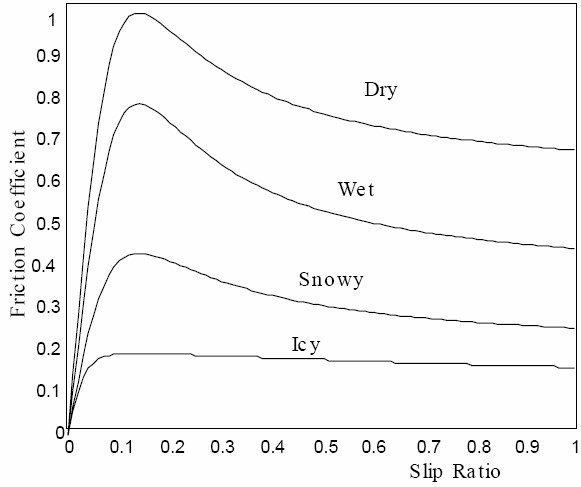
\includegraphics{image/friction coef.jpeg}
    \caption{Friction Coefficients in different conditions.}
    \label{fig:friction_coef}
\end{figure}

In the real world conditions, these parameters are really hard to measure or estimate because they change based on the road conditions (see Figure~\ref{fig:friction_coef}).

The real parameters of the vehicle in the simulation environment have been found with the help of Carla's \texttt{Vehicle.physics} command.

\medskip
\noindent\textbf{Vehicle Parameters Values}
\begin{itemize}
    \item $m$: 1318\,kg
    \item $J$: 2500\,kg/m\textsuperscript{2}
    \item $l_f$: 1.54\,m
    \item $l_r$: 1.51\,m
    \item $c_f$: 15000\,N/rad
    \item $c_r$: 15000\,N/rad
\end{itemize}

\subsection{Dispatching To Obtain Throttle-Brake Value From Acceleration Value}
To control a vehicle in the Carla simulator, we need three pieces of information: steering angle, throttle, and brake commands. However, our model generates $a_x$ data. It is not possible to directly provide this data to Carla because this information only tells us about the acceleration or deceleration of the vehicle and the magnitude of these changes. Therefore, we need to scale this data to use it for throttle-brake information. To do this, we perform dispatching. In the context of control, \enquote{dispatching} usually refers to the process of distributing tasks or resources according to certain criteria or algorithms.

To accomplish this, we first need specific reference values. These reference values should be collected according to many different scenarios to ensure they are suitable for every scenario, not just one. In our case, data were collected for three different scenarios: when the vehicle completes a straight path in a sine wave pattern, when continuous braking and accelerating are performed on a straight road, and finally, when only accelerating is done and the vehicle slows down without braking due to its own weight. The data include the vehicle's $a_x$ acceleration value, and throttle and brake values. By examining these accelerations, the priorities of throttle and brake values are determined for acceleration and deceleration situations. For instance, it is not always necessary to brake for negative acceleration values; reducing the throttle can also achieve the necessary speed reduction. Therefore, each value has its weight. Also, there is a range within which each command should be applied. These ranges can be determined using an if/else structure based on the acceleration value. The commands to be applied within these ranges are found by dividing the $a_x$ value by certain weight values. Consequently, the throttle and brake values are instantaneously derived from the $a_x$ value and provided to the vehicle in the Carla environment for application. As explained above, these values were found by analyzing reference data and through trial and error. The code for the if/else structure that creates the intervals for applying these values and commands is provided below.

\section{Data Gathering with Autonomous Driving Mode}
A reference point was selected from the Carla Map to collect reference data. The vehicle was spawned at this reference point. A simulation duration was determined based on a finish point we had predetermined. The vehicle was moved using Carla's autonomous driving mode. During this time, the necessary reference position, waypoint data, yaw angle, and speed data were recorded into a \texttt{.csv} file at intervals of $T_s = 0.05$ seconds. Once the required simulation duration was completed, the vehicle was removed from the map.
\hyphenation{}
Two collector routines are used during the recording. The first one, \texttt{carla\_data\_collector}, queries the full localization information of the vehicle at every tick: world position $(x, y, z)$, rotation (pitch, yaw, roll), linear velocity, linear acceleration and angular velocity. The second one, \texttt{carla\_data\_collector\_2}, focuses on the geometry of the lane and returns, for each tick, the position of the closest waypoint together with the unit forward vector $\hat{t} = (t_x, t_y)$ tangent to the lane in the legal direction of travel. The two collectors are complementary: the first one captures the dynamic state of the ego vehicle, the second one captures the geometric reference that the lane-keeping controller will track. The complete listings of both routines are reported in Appendix~\ref{app:b} for completeness; here we only describe the meaning of the recorded fields.

In order to keep the resulting \texttt{.csv} file compact, the second collector is wrapped by a duplicate-suppression block. The position of the closest waypoint can remain unchanged for several consecutive ticks---for instance when the vehicle stops at a traffic light---and writing identical rows to the file would simply increase its size without adding information. The block compares each new sample with the last one written and appends it only if at least one of the two coordinates has changed. The resulting file therefore contains a strictly monotonic sampling of the center line, indexed by the order in which the waypoints were visited.

\section{Data Gathering with Manual Driving Mode}
The first capability that we demonstrate with CARLA is localization, which allows our ego-vehicle to determine its pose in the world. Two coordinate frames: the map frame, which is a coordinate frame that is fixed at the initial position of the map, and the vehicle frame, which is a coordinate frame attached to the middle of the rear axle of the vehicle. For our particular experiment, we record the vehicle's accurate pose while traversing a curved-straight route in the Town10. In the Python API, there is a class that comprises all the localization information for an actor at a certain moment in time; its methods comprise Getters such as \texttt{get\_acceleration}, \texttt{get\_velocity}, \texttt{get\_transform}, and \texttt{get\_angular\_velocity}---which in our case we utilize the \texttt{get\_transform} method which includes both location of the object ($X$, $Y$, $Z$ from the origin of the map) in meters, and its rotation characteristics from which we utilize the yaw values. More concisely, $X$ and $Y$ coordinates were our focus, as in the map chosen, the road is entirely flat. Hence only these two coordinates remain crucial for tracking the vehicle's trajectory. Also, the Yaw angle, describing the orientation of the map's coordinate system, is essential for indication of the direction the vehicle is facing. Therefore for curved paths, which our scenarios contain, it is important.

Some additional considerations also are to be noted, such as the sampling rate, which determines the time step of the data collection. We have chosen $0.1$, indicating not too sparse to miss some critical dynamics, especially for sharp turns, and also not too frequent leading to redundant information.

After initializing the scenario and ego vehicle (based on the preferences), based on the duration of the scenario depending on the controls of the car (throttle, brake, and steering commands), we record the data of the vehicle at each time step. The corresponding logging routine has the same overall structure as in the autonomous mode---at every simulation tick the snapshot frame, the pose, the velocity, the acceleration and the applied control are appended to a Pandas dictionary which is finally written to disk as a \texttt{.csv} file. The full code excerpt is provided in Appendix~\ref{app:b}.
\hyphenation{}
In manual driving mode, the autopilot is disengaged with \texttt{vehicle.set\_autopilot(False)} and the user is given full control of throttle, brake, and steering through the keyboard. Each pressed key is captured as a PyGame event and is translated into a \texttt{carla.VehicleControl} object that is then applied to the ego vehicle in the simulator. While the user drives, the same getters introduced for the autonomous mode are queried at every simulation tick, so that the resulting \texttt{.csv} file shares the same structure for both modes and can be loaded by the controller without any additional preprocessing.

This dual-mode acquisition serves two purposes. First, it provides reference trajectories for the dispatcher tuning and for the controller design, since the autonomous mode of CARLA produces well-formed paths along the center of the lane. Second, it allows the recording of edge cases that are hard to reproduce automatically---for example aggressive lane changes, harsh braking, or following curves at the limit of stability---because they can be performed deliberately by a human driver. The two \texttt{.csv} files are then used as the input data set for the \ac{LKA} controller described in Chapter~\ref{ch3}.
\chapter{Lane Keeping Assist: Theory, Architectures and Method Comparison}
\label{ch3}

% chapters/chapter4.tex  — converted from chapter4.typ
% Conventions used (identical to chapter1.tex / chapter2.tex / chapter3.tex):
%   Typst @KEY            -> \ac{KEY}            (auto: long on first use, short after)
%   Typst @KEY:lo         -> \acl{KEY}          (long form only)
%   Typst @figlabel       -> Figure~\ref{fig:figlabel}
%   Typst @tablabel       -> Table~\ref{tab:tablabel}
%   Typst @sec_label      -> Section~\ref{sec:label}
%   Typst @chN            -> Chapter~\ref{chN}
%   Typst @eqt:eq_label   -> Equation~\eqref{eq:label}
%   Typst @citekey        -> \cite{citekey}
%   Typst `code`          -> \texttt{code}      (underscores and & escaped)
%   Typst _italic_        -> \emph{italic}
%   Typst "quoted"        -> \enquote{quoted}
% The Typst `#import "functions.typ"` has no LaTeX counterpart and is dropped.
%
% NOTE: cross-refs resolve against labels defined in chapter3.tex
%       (sec:sysid, sec:vision, eq:lane_shift, tab:arch_summary) and against
%       \label{ch2}, \label{ch3}. They are all present in the converted chapters.

\chapter{Simulation Results and Evaluation}
\label{ch4}

The previous chapter developed three lateral-control architectures for the \ac{LKA} function and motivated each design choice on control-theoretic grounds. The present chapter complements that theoretical discussion with the numerical evaluation of the three controllers in CARLA. All experiments are run on the same test route in Town06, with the same vehicle (\texttt{vehicle.nissan.patrol}), the same target speed of $30$~km/h, the same simulation rate $T_s = 0.05$~s, and the same set of PID gains obtained from the system-identification procedure of Section~\ref{sec:sysid}. Under these conditions, any observed difference between the trajectories can be attributed to the structure of the error signal and to the corresponding controller rather than to incidental variations in the simulator.

The chapter is structured as follows. Section~\ref{sec:exp_setup} describes the experimental protocol, the reference path and the metrics used to compare the controllers. Section~\ref{sec:carla_view} presents a qualitative view of the test route as rendered inside the CARLA world. Section~\ref{sec:full_traj} quantifies the tracking performance over the entire route. Section~\ref{sec:smooth_turn} and Section~\ref{sec:lane_change} then zoom in on two representative sections of the route---the long smooth curve and a sudden lane discontinuity---where the differences between the three architectures become most visible. Section~\ref{sec:discussion} finally interprets the results in the light of the control-theoretic predictions of Chapter~\ref{ch3}.

\section{Experimental Setup}
\label{sec:exp_setup}
The reference path was recorded once, in autopilot mode, by driving the ego vehicle through Town06 and logging the closest waypoint at every simulation tick, as described in Chapter~\ref{ch2}. The resulting \texttt{carla\_data.csv} file contains a strictly monotonic sampling of the center line along an approximately $L$-shaped route of about $850$~m. The route starts on a north--south urban street, executes a $90^\circ$ left turn onto a long east--west arterial, and ends after a stretch of straight road that includes a step-like lane discontinuity---a feature that proves particularly informative when comparing the three controllers. The route was selected because it exercises both the steady-state behavior of the controllers, on the long straight section that follows the turn, and their transient behavior, on the corner itself and on the lane discontinuity.

Three closed-loop experiments were then performed on this same route, one for each architecture:

\begin{itemize}
    \item \emph{Cross-track PID} (\texttt{lane\_shift\_pid/pygame\_controller.py}). The reference is the recorded path; the error is the cross-track distance Equation~\eqref{eq:lane_shift}; the controller is a full PID with the gains $K_p, K_i, K_d$ produced by \texttt{pid\_tuning.py} for $\omega_n^{\mathrm{lat}} = 1.5$~rad/s. The trajectory is logged to \texttt{ego\_trajectory\_shift.csv} and appears in blue on every plot of this chapter.
    \item \emph{Heading-error PI} (\texttt{heading\_error\_pid/pygame\_controller.py}). The reference is again the recorded path, but the error is the look-ahead heading angle; the controller is a PI with the gains produced by \texttt{pid\_tuning.py} for $\omega_n^{\mathrm{lat}} = 2.0$~rad/s. The trajectory is logged to \texttt{ego\_trajectory\_heading.csv} and appears in green.
    \item \emph{Vision-based PI} (\texttt{detection\&pid.py}). The reference is reconstructed at every tick from the RGB camera by the CLRNet lane detector~\cite{clrnet} followed by the \acs{IPM} projection of Section~\ref{sec:vision}. The same PI controller of the previous architecture consumes the heading error computed in the body frame. At intersections the \ac{LKA} hands off to the CARLA Traffic Manager autopilot, as described in Section~\ref{sec:vision}. The trajectory is logged to \texttt{ego\_trajectory\_vision.csv} and appears in red.
\end{itemize}

The longitudinal channel is identical in the three experiments: a discrete PI regulator drives the speed to $30$~km/h with the gains obtained from the longitudinal step experiment of Section~\ref{sec:sysid}. All three trajectories are post-processed by \texttt{plot\_trajectory.py}, which overlays the recorded reference path and computes two scalar performance metrics:

\begin{itemize}
    \item The \emph{\acl{RMSE}}, \ac{RMSE} $e_y = \sqrt{(1/N) \sum_{k=1}^N e_y[k]^2}$, which summarizes the average tracking accuracy over the run;
    \item The \emph{maximum absolute cross-track error}, $\max \lvert e_y \rvert = \max_{k} \lvert e_y[k] \rvert$, which captures the worst-case excursion from the center of the lane.
\end{itemize}

For the vision-based run, the cross-track error reported by the plotting script is computed \emph{a posteriori} against the same recorded reference path used by the other two runs, even though the controller itself never has access to that path. This makes the three runs comparable on a common metric and isolates the effect of the perception layer from the rest of the control loop. It is also worth stressing that the cross-track error used here as a comparison metric is \emph{not} the error signal of the heading-error and vision-based controllers: those two controllers close their loop on an angle, and the cross-track distance is only computed \emph{off-line} for evaluation purposes.

\section{Qualitative View in CARLA}
\label{sec:carla_view}
Before turning to the numerical metrics, it is useful to look at the test route as it appears in the simulator itself. The script \texttt{draw\_trajectory\_in\_carla.py} takes a logged trajectory and draws it as a coloured line directly in the CARLA world, on top of the textured road, using the simulator's debug-drawing API. The start of the trajectory is marked with a green sphere and the end with a red sphere. Figure~\ref{fig:traj_carla} reproduces one of these renderings for the heading-error PI run, which is the controller that achieves the best tracking accuracy over the full route.

\begin{figure}[htbp]
    \centering
    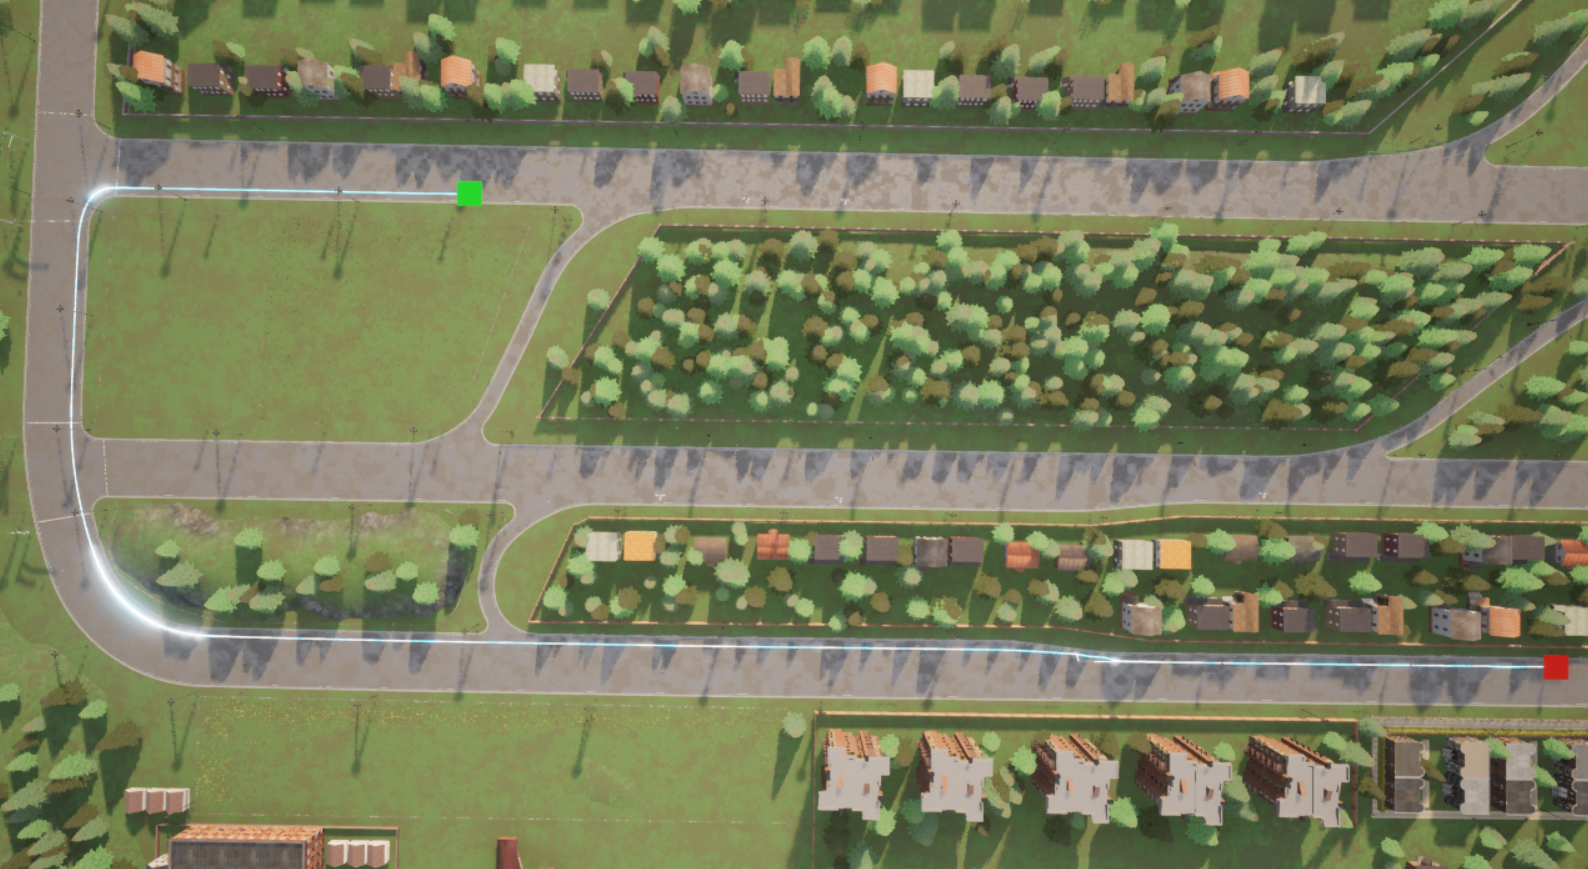
\includegraphics[width=0.8\linewidth]{image/fig_trajectory_in_carla.png}
    \caption{Top-down view of Town06 with the trajectory of the heading-error PI controller drawn in cyan by \texttt{draw\_trajectory\_in\_carla.py}. The green square marks the start of the run, the red square marks the end. The vehicle enters from the top of the figure, executes a $90^\circ$ left turn at the intersection, and proceeds east along the arterial. The line stays well inside the lane throughout the manoeuvre, which is the basic visual confirmation that the controller fulfils its \acs{LKA} purpose. The remaining discussion of this chapter focuses on the quantitative differences between the three architectures along this same route.}
    \label{fig:traj_carla}
\end{figure}

Two observations can already be made from the in-simulator view. First, the trajectory stays well inside the lane throughout the manoeuvre---the rendered line never leaves the asphalt and remains close to the center of the lane on both the curved and the straight sections of the route. This is the minimum requirement for a \ac{LKA} and the most basic safety check. Second, the corner itself is the most demanding part of the route: it concentrates a large change in the reference heading into a short stretch of road and produces the largest transients in the cross-track error, as the next section will show.

\section{Full-Route Tracking Performance}
\label{sec:full_traj}
The first quantitative comparison is performed over the entire route. Figure~\ref{fig:traj_full} shows the top-down trajectory plot (left) and the cross-track error as a function of time (right), with the three controllers overlaid on the same axes and with the \ac{RMSE} and maximum absolute error reported in the legend.

\begin{figure}[htbp]
    \centering
    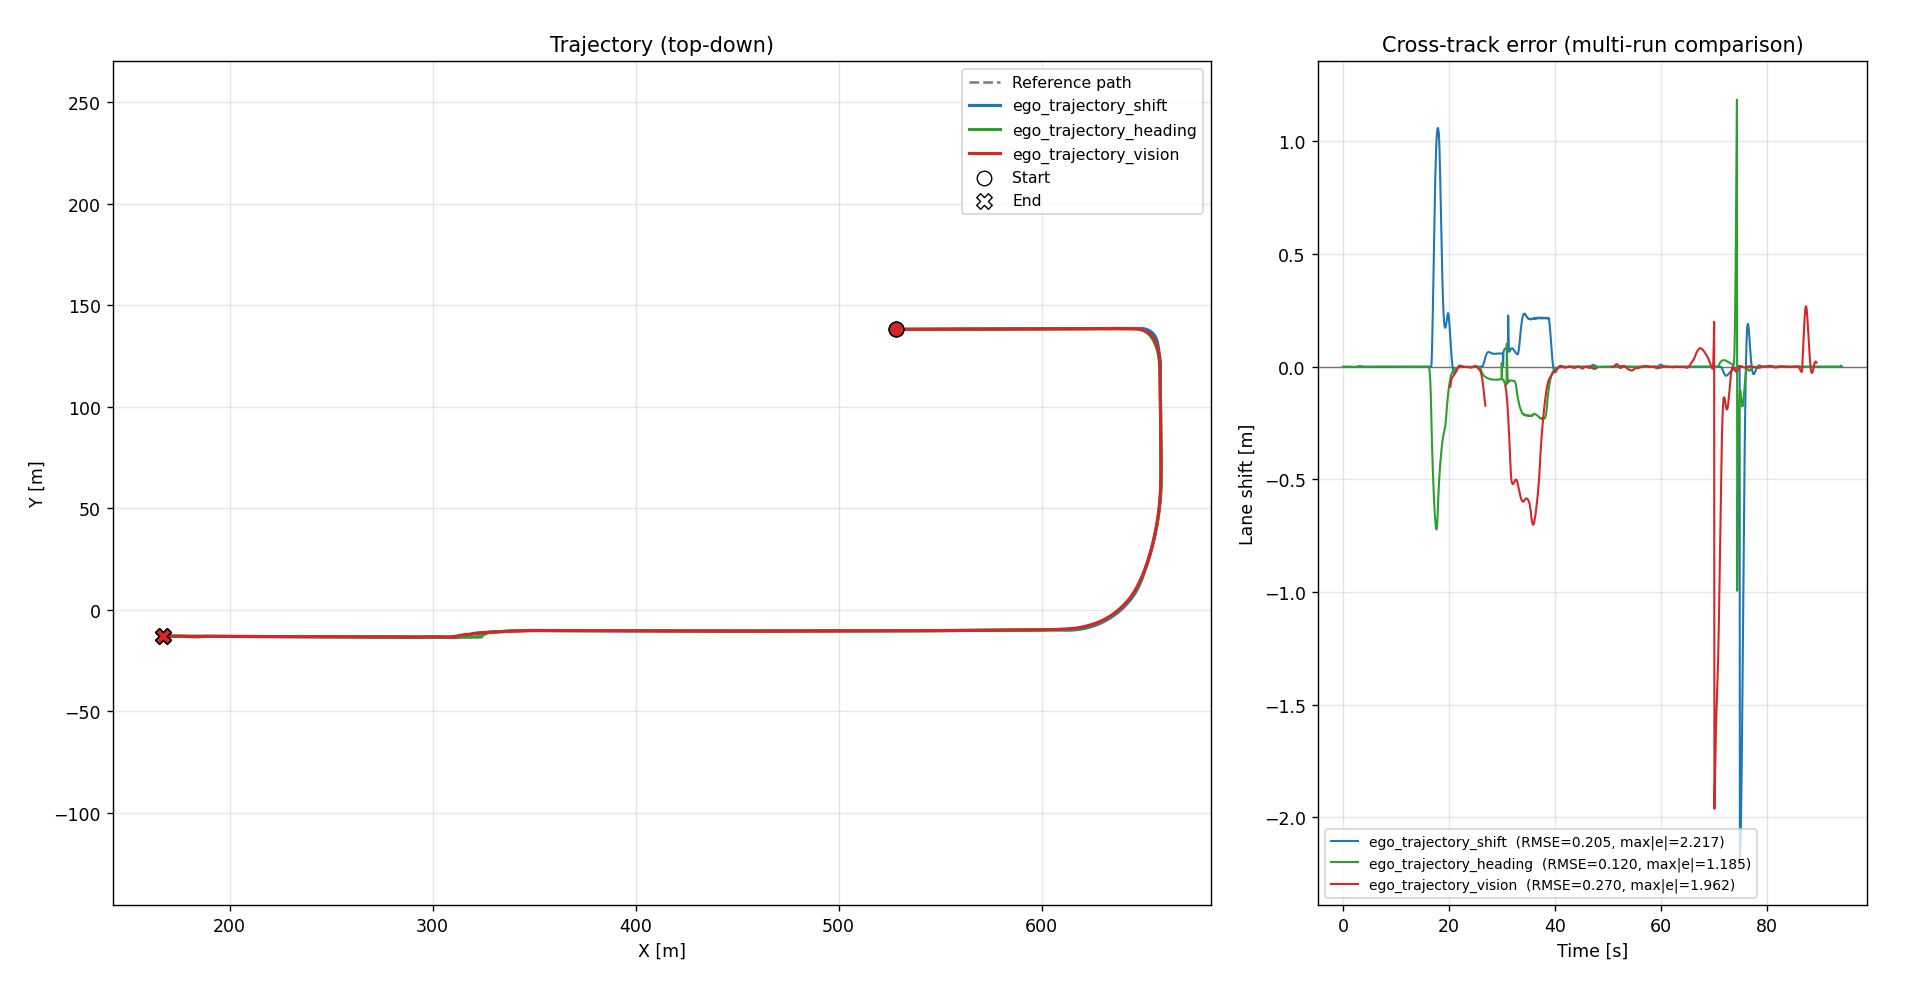
\includegraphics[width=\linewidth]{image/fig_trajectory_full.png}
    \caption{Full-route comparison of the three controllers. \emph{Left}: top-down view of the recorded reference path (grey dashed) and of the three closed-loop trajectories (cross-track PID in blue, heading-error PI in green, vision-based PI in red). Start and end of each run are marked with circles and crosses respectively. \emph{Right}: cross-track error $e_y(t)$ as a function of time, with the root-mean-square error and the maximum absolute error reported in the legend. The two large transients around $t \approx 18$--$22$~s and $t \approx 70$--$75$~s correspond respectively to the $90^\circ$ corner and to a step-like lane discontinuity in the reference path.}
    \label{fig:traj_full}
\end{figure}

A few comments on the figure. On the long straight section that follows the corner---roughly from $t \approx 25$~s to $t \approx 60$~s---the three trajectories are visually indistinguishable from the reference at the scale of the left-hand panel, even though small but persistent biases are visible on the right-hand error trace. These steady-state biases are the subject of Section~\ref{sec:smooth_turn}. The two large excursions occur at the $90^\circ$ corner, where the cross-track and the vision-based controllers overshoot by approximately $1$~m, and at the step-like lane discontinuity around $t \approx 70$--$75$~s, where the maximum excursions of the run are recorded. Note that the cross-track error trace of the vision-based controller has a finite duration: the controller starts logging only once the lane detector returns a valid center line, which is the reason why the red curve is missing on the very first seconds of the trace.

The numerical metrics extracted from the right-hand panel are summarized in Table~\ref{tab:full_metrics}. The heading-error PI achieves both the lowest \ac{RMSE} and the lowest maximum excursion of the three architectures, by a clear margin. The cross-track PID is intermediate in \ac{RMSE} but exhibits the worst maximum excursion of the three runs at the lane discontinuity. The vision-based PI has the highest \ac{RMSE}, mainly because of a persistent steady-state bias on the smooth curve that the next section will analyze in detail.

\begin{table}[htbp]
    \centering
    \footnotesize
    \begin{tabular}{@{} l c c l @{}}
        \toprule
        \textbf{Controller} & \textbf{\acs{RMSE} $e_y$ [m]} & \textbf{$\max \lvert e_y \rvert$ [m]} & \textbf{Worst-case event} \\
        \midrule
        Cross-track PID  & $0.205$ & $2.217$ & Step-like lane discontinuity \\
        \addlinespace
        Heading-error PI & $0.120$ & $1.185$ & Step-like lane discontinuity \\
        \addlinespace
        Vision-based PI  & $0.270$ & $1.962$ & Step-like lane discontinuity \\
        \bottomrule
    \end{tabular}
    \caption{Tracking metrics over the entire route, read directly from the legend of Figure~\ref{fig:traj_full}. Lower is better.}
    \label{tab:full_metrics}
\end{table}

The relative ordering of the three controllers---heading-error best, cross-track intermediate, vision-based worst on \ac{RMSE}---matches the qualitative prediction of Table~\ref{tab:arch_summary} on the structural argument (heading-error preferred over cross-track because of the lower plant order) but adds a new piece of information that the theoretical chapter could not anticipate: the perception layer of the vision-based controller introduces a steady-state bias on the smooth curve that dominates its \ac{RMSE}. The maximum-excursion ordering is different: there, the worst performer is the cross-track PID at $2.22$~m, with the vision-based PI at $1.96$~m and the heading-error PI at $1.19$~m. All three peaks coincide in time with the step-like lane discontinuity of the reference path, which is a deliberately adversarial test case discussed in Section~\ref{sec:lane_change}.

\section{Performance on a Smooth Curve}
\label{sec:smooth_turn}
The first zoom-in focuses on the long smooth curve that occurs after the corner, between $t \approx 25$~s and $t \approx 45$~s. The road curvature in this section is gentle and approximately constant, so the relevant figure of merit is the \emph{steady-state cross-track error} that each controller maintains while tracking a constant-curvature reference. Figure~\ref{fig:traj_smooth} shows the top-down trajectory (left) and the cross-track error (right) restricted to this section of the route.

Three quantitative observations can be made from Figure~\ref{fig:traj_smooth}. The cross-track PID (blue) settles to a positive steady-state error of approximately $+0.22$~m, which means that the vehicle rides on the \emph{outside} of the curve relative to the center line. This is the classical signature of a PID that is fighting a constant disturbance---the road curvature acts as a constant input to the lateral plant---and that has not yet had the time to absorb it through its integral term. The heading-error PI (green) settles to a negative steady-state error of approximately $-0.22$~m, which means that the vehicle rides on the \emph{inside} of the curve. The opposite sign of the two biases is a direct consequence of the different error signal: the cross-track controller tries to keep $e_y = 0$ at the closest waypoint, whereas the heading-error controller tries to keep the look-ahead angle $\alpha = 0$, and the look-ahead point on a curved reference is geometrically inside the curve relative to the closest waypoint. The two biases have similar magnitude but they reflect two different geometric definitions of \enquote{being on the center}.

\begin{figure}[H]
    \centering
    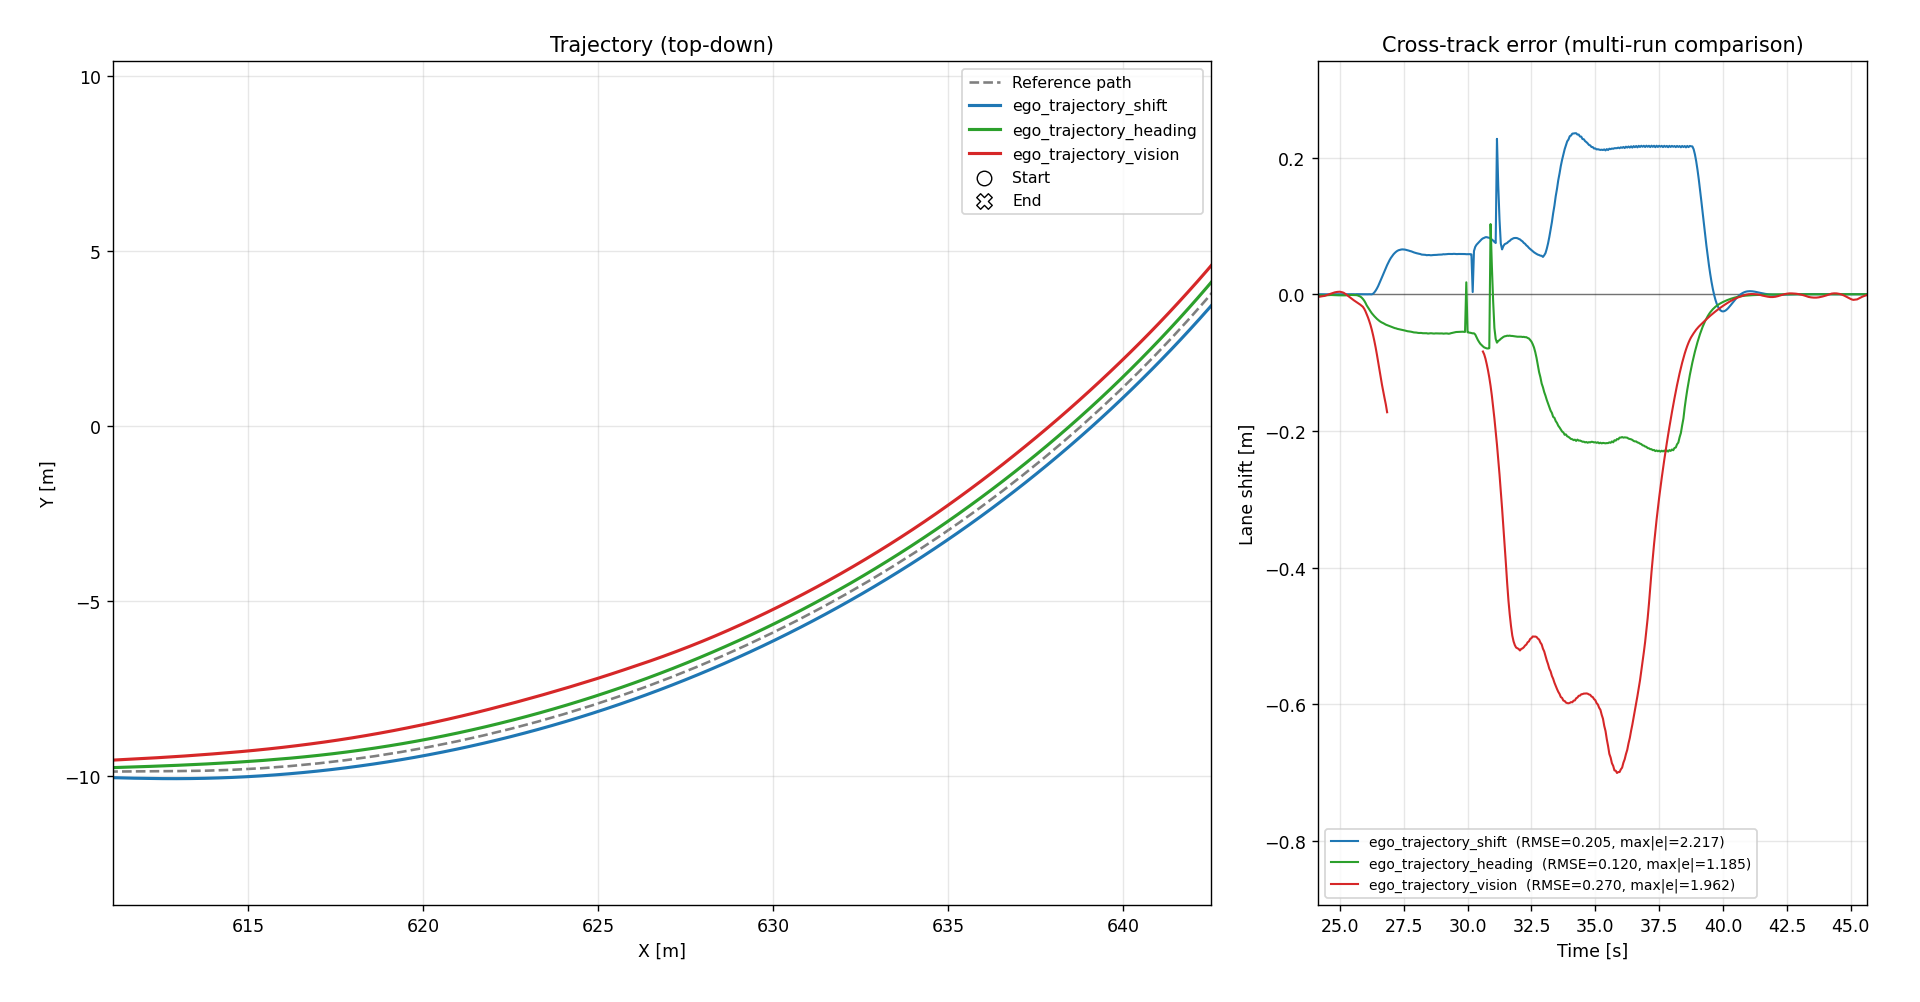
\includegraphics[width=\linewidth]{image/fig_trajectory_smooth_turn.png}
    \caption{Smooth-curve detail. \emph{Left}: top-down view of the recorded reference (grey dashed) and of the three closed-loop trajectories along a gentle, approximately constant-curvature stretch of road between $X \approx 615$~m and $X \approx 640$~m. The three controllers track the same curve with different signed steady-state biases that are clearly visible at this magnification. \emph{Right}: corresponding cross-track error between $t \approx 25$~s and $t \approx 45$~s. The vision-based PI exhibits a large negative bias that reaches $\approx -0.7$~m at the apex of the curve, while the cross-track PID and the heading-error PI settle to biases of opposite sign with comparable magnitude of $\approx +0.22$~m and $\approx -0.22$~m respectively.}
    \label{fig:traj_smooth}
\end{figure}

The vision-based PI (red) exhibits a much larger negative bias that reaches approximately $-0.7$~m at the apex of the curve, a factor of three larger than the heading-error PI on which it is built. The two controllers share the same control law and the same gains; the only difference is the source of the look-ahead point. The conclusion is that the additional bias is introduced by the perception layer. Two mechanisms contribute to it. First, the center line returned by \texttt{get\_centerline} is the average of the two \emph{detected} lane boundaries, which are themselves curved; the mid-point of two parallel arcs is biased toward the inside of the curve by an amount proportional to the curvature and to the lateral spacing between the boundaries. Second, the first-degree polynomial fit of Section~\ref{sec:vision} approximates a locally curved center line with a straight line, which systematically truncates the lateral component of the look-ahead target. Both mechanisms have the same sign and combine into the observed bias. On a straight road, neither mechanism is active and the vision-based controller behaves exactly like the heading-error PI, which is consistent with the near-zero error reported in Figure~\ref{fig:traj_full} before $t \approx 25$~s.

It is also worth noting that the magnitudes involved here---$0.22$~m for the path-based controllers and $0.7$~m for the vision-based controller---remain comfortably within the half-width of a typical CARLA lane, which is approximately $1.75$~m. The biases on the smooth curve therefore do not threaten the safety of the \ac{LKA} function; they only degrade the comfort and the tracking accuracy.

\section{Performance on a Sudden Lane Discontinuity}
\label{sec:lane_change}

\begin{figure}[H]
    \centering
    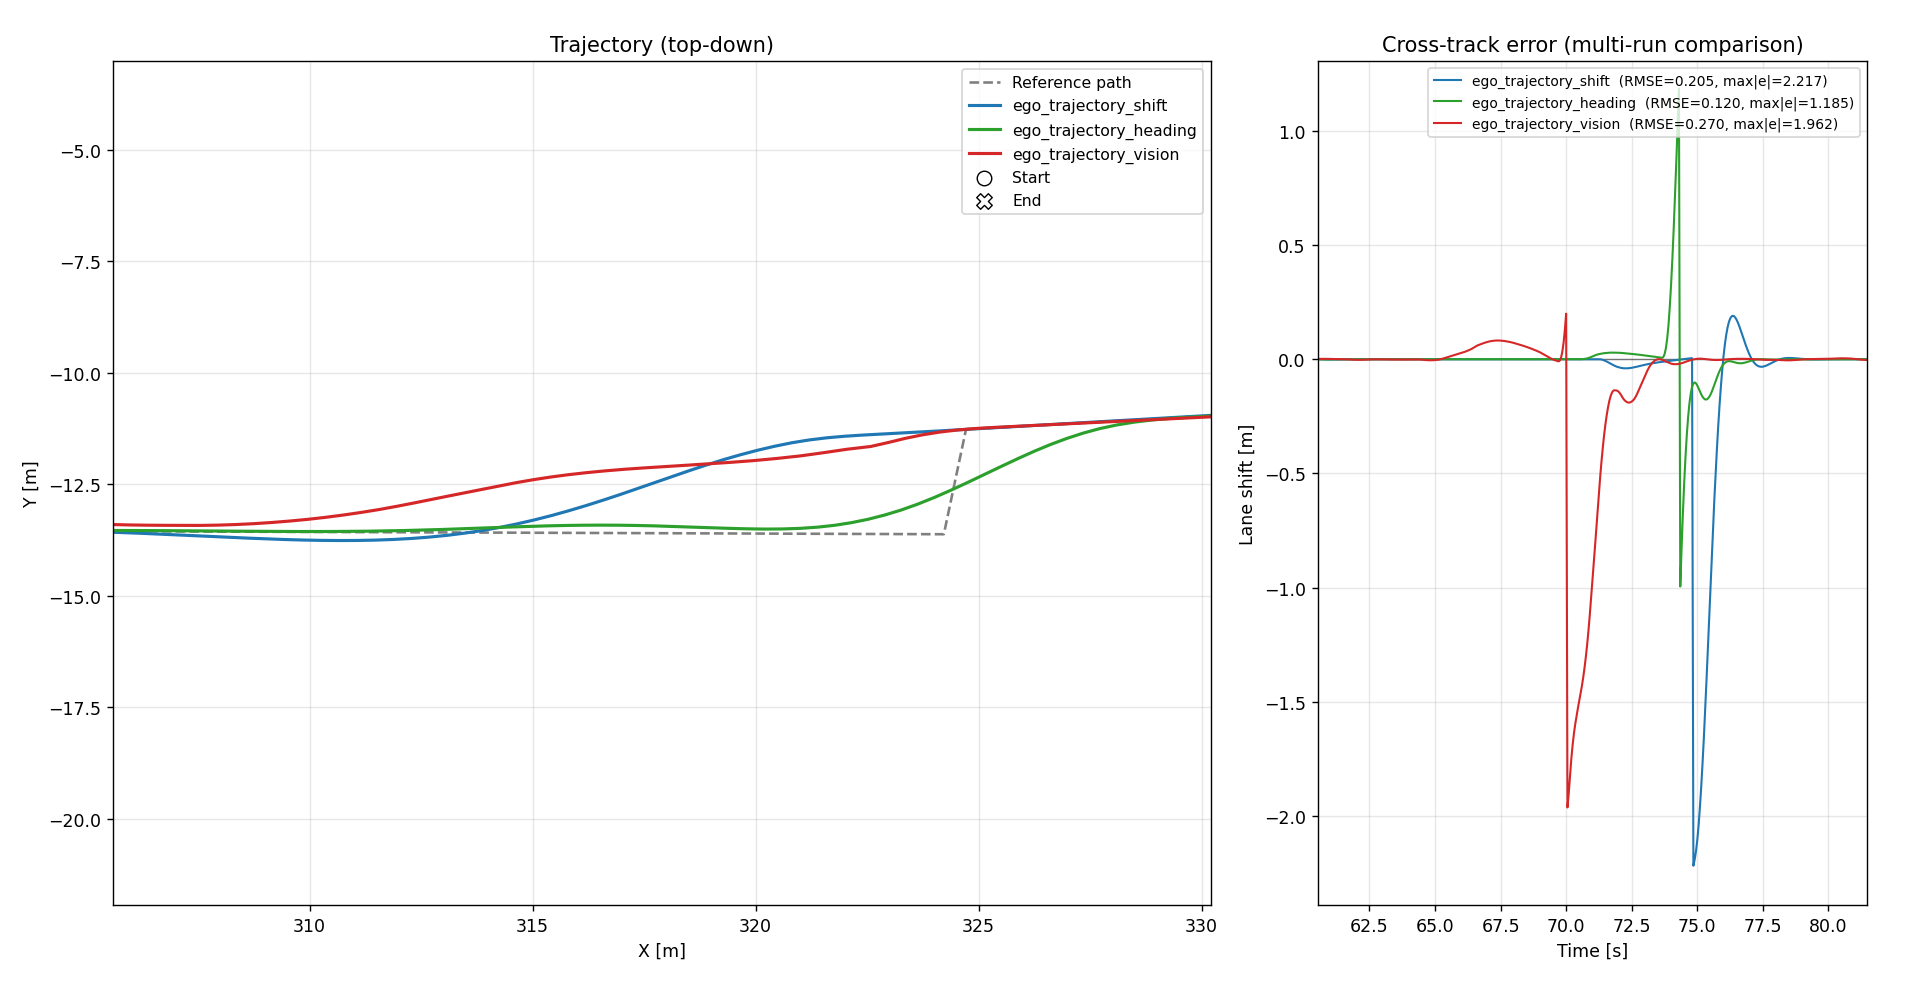
\includegraphics[width=0.85\linewidth]{image/fig_trajectory_lane_change.png}
    \caption{Step-like lane discontinuity. \emph{Left}: top-down view of the reference (grey dashed) and of the three closed-loop trajectories in the neighborhood of the discontinuity. The reference exhibits a step of approximately $3$~m at $X \approx 325$~m. The three controllers react with very different transients. \emph{Right}: cross-track error between $t \approx 60$~s and $t \approx 80$~s. The cross-track PID (blue) takes the largest excursion at $\approx -2.22$~m; the vision-based PI (red) anticipates the discontinuity and undershoots by $\approx -1.96$~m around $t \approx 70$~s; the heading-error PI (green) is the smoothest of the three, with a single overshoot of $\approx +1$~m.}
    \label{fig:traj_change}
\end{figure}

The second zoom-in focuses on a step-like discontinuity of the reference path that occurs around $t \approx 70$--$75$~s, which corresponds to the right-hand spikes visible in Figure~\ref{fig:traj_full} and which is shown in detail in Figure~\ref{fig:traj_change}. This discontinuity is an artefact of the way the reference path was recorded: when the vehicle in autopilot mode merged from one lane into an adjacent one, the closest-waypoint logger jumped from the center line of the first lane to the center line of the second one, which produces a step of approximately one lane width ($3$~m) in the reference. From the controller's point of view, this is the worst possible kind of disturbance: a step in the reference rather than a step in the disturbance input.

The three controllers react to the step in three qualitatively different ways. The cross-track PID (blue) follows the original lane up to the discontinuity, then suddenly sees a large positive cross-track error appear on its closest waypoint and reacts with a large steering input that overshoots the new lane by $\approx 2.2$~m on the opposite side. This is the worst-case event of the whole run for this controller, and it is the manifestation of the limited phase margin of the cross-track loop: a step on the input of a double integrator is integrated twice before the controller has any chance to react, and the resulting overshoot is bounded only by the rate-limited saturation of the steering actuator. The transient takes approximately $2$~s to decay.

The heading-error PI (green) reacts differently. The look-ahead point is, by construction, several meters ahead of the vehicle; the controller therefore \enquote{sees} the discontinuity coming and starts steering toward the new lane before the discontinuity is reached. The cross-track error in Figure~\ref{fig:traj_change} shows a much smaller positive transient of approximately $+1$~m, followed by a small undershoot of $-1$~m as the look-ahead point crosses the step in the opposite direction. The transient is over within a single look-ahead time horizon, that is in less than $1$~s. The maximum-excursion metric on this controller is the smallest of the three at $1.19$~m, which is essentially this single peak.

The vision-based PI (red) reacts earliest of all three because the lane detector reconstructs the upcoming center line several meters ahead of the vehicle and the polynomial fit smooths the discontinuity into a gradual lateral shift. The cross-track error trace shows a large negative excursion that starts at $t \approx 67$~s---well before the path-based controllers react---and reaches $\approx -2$~m at $t \approx 70$~s. This is \emph{not} a tracking failure: the vehicle is correctly following what the camera sees, and what the camera sees is a smooth lateral shift rather than a step. The error is large because the metric is computed against the path-based reference, which itself contains the step. In a real-world deployment, where the only reference is the camera image, this trajectory would actually be the smoothest and the most natural-feeling of the three.

The lane-discontinuity event therefore illustrates the fundamental difference between the three approaches: the path-based controllers track a pre-recorded reference and are penalized by any discontinuity in that reference, while the vision-based controller tracks what is actually painted on the road and can naturally absorb such discontinuities at the cost of an inevitable lag with respect to a discontinuous ground-truth metric.

\section{Discussion}
\label{sec:discussion}
The numerical results of this chapter both confirm and refine the control-theoretic predictions of Chapter~\ref{ch3}. The reduction of one plant integrator from the cross-track to the heading-error formulation buys a measurable improvement in tracking accuracy: the heading-error PI achieves an \ac{RMSE} of $0.120$~m against the $0.205$~m of the cross-track PID, a factor of $1.7$ improvement, and a maximum excursion of $1.19$~m against $2.22$~m, a factor of $1.9$ improvement. Both numbers are consistent with the larger phase margin and the gentler gain schedule that Table~\ref{tab:arch_summary} attributed to the heading-error formulation.

The addition of a perception layer on top of the heading-error PI is less clear-cut. On a straight road, the vision-based controller is indistinguishable from its path-based counterpart, as expected. On a smooth curve, the perception layer introduces a steady-state bias of approximately $-0.7$~m that the controller cannot remove because it never sees the path-based reference. This bias is the price to pay for being independent of a pre-recorded map. On a step-like lane discontinuity, the perception layer is actually beneficial because it smooths the discontinuity into a gradual lateral shift; the large excursion that appears on the cross-track error metric is an artefact of the comparison against a discontinuous reference, not a tracking failure of the controller.

A subtler point is the role of the controller speed of reaction. The heading-error PI uses a look-ahead distance of $L_d \approx 9$~m at $30$~km/h, which gives the controller approximately $1$~s of preview on the reference. The vision-based PI uses the same preview horizon but applies it to a perception-based reference. The cross-track PID has no preview at all: it reacts to the closest waypoint, which is by definition the present, not the future. The factor of $1.9$ on the maximum excursion between the cross-track and the heading-error controllers is therefore not only a consequence of the lower plant order, but also of the implicit feed-forward that the look-ahead introduces. Disentangling the two effects would require an additional experiment in which the cross-track PID is augmented with an explicit feed-forward term computed from the road curvature; this is left for future work.

From a practical standpoint, the experiments support the following recommendations for an \ac{LKA} function deployed in this kind of simulation environment. The cross-track PID is the simplest of the three architectures to implement and tune, but it is the most sensitive to discontinuities in the reference and to changes in the vehicle speed; it is acceptable for low-speed, smooth-path applications. The heading-error PI is the most accurate and the most robust to reference discontinuities; it is the recommended choice whenever a pre-recorded reference path is available. The vision-based PI is the only one of the three that does not depend on a pre-recorded map; it pays for this independence with a steady-state bias on curves, which can be mitigated either by a higher-order polynomial fit of the center line or by a curvature-aware correction of the look-ahead point. The detailed implementation of these mitigations is the subject of the chapter on future work.

The next chapter draws the overall conclusions of the thesis and outlines the directions for future investigation.

% chapters/chapter5.tex  — converted from chapter5.typ
% Conventions used (identical to chapter1–4.tex):
%   Typst @KEY            -> \ac{KEY}            (auto: long on first use, short after)
%   Typst @chN            -> Chapter~\ref{chN}
%   Typst @sec_label      -> Section~\ref{sec:label}
%   Typst @citekey        -> \cite{citekey}
%   Typst `code`          -> \texttt{code}      (underscores and & escaped)
%   Typst _italic_        -> \emph{italic}
% The Typst `#import "functions.typ"` has no LaTeX counterpart and is dropped.
%
% NOTE: cross-refs reach into other chapters and resolve against labels already
%       defined there: \ref{ch1}, \ref{ch2}, \ref{ch4} (chapter1/2/4.tex) and
%       sec:bicycle, sec:heading, sec:sysid (chapter3.tex). All are present.

\chapter{Conclusions and Future Work}
\label{ch5}

This thesis has investigated the implementation and evaluation of a \ac{LKA} function inside a software-only \ac{VIL} simulation environment based on the CARLA simulator. The work spans the full chain from the selection of the simulation platform, through the modelling and the system identification of the vehicle, to the design of three progressively richer lateral-control architectures and to their numerical evaluation on a common test route. The present chapter summarizes the main findings of the previous chapters, restates the contributions of the work, and outlines the directions in which the present results could be extended.

\section{Summary of the Work}
The thesis is articulated into four substantive chapters that build on each other in a clear progression from environment selection to controller evaluation.

Chapter~\ref{ch2} has selected CARLA as the simulation platform of the work, motivated by its open-source nature, its Unreal-Engine-4-based rendering, its accurate physics engine, and---most importantly for the present application---its comprehensive Python API. The same chapter has introduced the \acs{DST} bicycle model that underlies the controller design and has explained how the vehicle parameters $m, J, l_f, l_r, c_f, c_r$ have been read from the CARLA blueprint of the chosen \texttt{vehicle.nissan.patrol}. A dispatching procedure that converts the analytical longitudinal acceleration into the throttle/brake commands accepted by the simulator has been described, together with a dual-mode data-gathering pipeline---autopilot for reference paths, manual driving for edge cases---that produces the \texttt{.csv} files consumed by the controllers.

Chapter~\ref{ch3} has developed the lateral-control component of the \ac{LKA} function in three progressively richer architectures. The cross-track PID closes the loop on the perpendicular distance between the vehicle and a pre-recorded reference path; the corresponding plant is a double integrator and a full PID is required for stability. The heading-error PI closes the loop on the angle between the vehicle's forward direction and a look-ahead point on the same reference path; the corresponding plant is a single integrator and a PI controller is sufficient. The vision-based PI replaces the pre-recorded reference with a center line reconstructed at every tick from the RGB camera by the CLRNet lane detector~\cite{clrnet} and by an \acs{IPM} projection; the same PI controller of the heading-error formulation consumes the heading error computed in the body frame. A pole-placement procedure derives the PID gains analytically from a measurement of the steering gain $K_{\mathrm{steer}}$ obtained by an open-loop step experiment on the simulator, and predicts that the heading-error formulation should be both more accurate, on a per-bandwidth basis, and more robust to changes in the vehicle speed.

Chapter~\ref{ch4} has evaluated the three architectures on a common test route in Town06. The numerical results have confirmed the predictions of the theoretical chapter on the relative ordering of the path-based controllers: the heading-error PI achieves an \ac{RMSE} of $0.120$~m and a maximum excursion of $1.185$~m against the $0.205$~m and $2.217$~m of the cross-track PID, an improvement by a factor of approximately $1.7$ on the average and of approximately $1.9$ on the worst case. The vision-based PI has achieved an \ac{RMSE} of $0.270$~m, which is larger than both path-based controllers; the increase is dominated by a steady-state bias of approximately $0.7$~m on the smooth curve, which has been traced back to two specific approximations of the perception layer---the geometric bias of the midline reconstruction and the first-degree polynomial fit of the center line. On a step-like lane discontinuity, the vision-based controller has been shown to react earlier than the path-based controllers and to produce the smoothest trajectory, at the cost of a large \emph{apparent} error against the discontinuous path-based reference.

\section{Contributions}
The original contributions of this thesis can be summarized as follows.

\begin{itemize}
    \item A modular, software-only \ac{VIL} implementation of a \ac{LKA} function in the CARLA simulator, in which the controller runs as an external Python process and communicates with the simulator through the synchronous-mode Python API at $20$~Hz. The code is organized into three self-contained modules---\texttt{lane\_shift\_pid/}, \texttt{heading\_error\_pid/}, and the vision-based \texttt{detection\&pid.py}---that share the same actuator, the same vehicle, and the same simulation rate, so that any observed difference between them can be attributed to the structure of the controller rather than to incidental implementation details. The complete source tree is publicly available in the open-source repository \texttt{LaneDetCarla}~\cite{lanedetcarla}, which accompanies this thesis.
    \item A complete, reproducible system-identification procedure (\texttt{carla\_sysid.py} and \texttt{pid\_tuning.py}) that fits the parameters of a first-order longitudinal model and a one-parameter lateral steering gain from two open-loop step experiments, and derives analytical PID gains by pole placement on the resulting plants. The procedure is fully automatic and produces ready-to-use Python dictionaries for the controllers.
    \item A side-by-side comparison of three lateral-control architectures of increasing sophistication, including a detailed control-theoretic analysis (plant order, gain scheduling, phase margin) and a numerical evaluation on a common test route with two scalar metrics. The comparison isolates, for the first time in this specific simulation setup, the contribution of the perception layer from the contribution of the controller structure.
    \item A vision-based \ac{LKA} controller that combines a state-of-the-art lane-detection network~\cite{clrnet} with an \acs{IPM} projection and with the same heading-error PI of the path-based architecture. The vision-based controller is shown to be a viable \ac{LKA} implementation that does not require any pre-recorded reference path, at the cost of a steady-state bias on curves that has been quantitatively characterized.
    \item An explicit junction-handling logic that detects intersections through the CARLA waypoint graph and hands the control over to the Traffic Manager autopilot for the duration of the junction, with a clean reset of the PI controller state at every re-engagement. This makes it possible to run the vision-based \ac{LKA} on routes that include intersections, which would otherwise be unmanageable for a vision-only formulation.
\end{itemize}

\section{Limitations}
The work also has limitations that should be acknowledged.

The evaluation is restricted to a single vehicle, a single map (Town06) and a single target speed ($30$~km/h). The gain-scheduling analysis of Section~\ref{sec:heading} predicts that the heading-error PI is robust to speed variations in the range $20$--$60$~km/h, but this prediction has not been verified experimentally; the same is true of the robustness to vehicle parameters. A systematic sweep over speed, vehicle and map would strengthen the generalizability of the results.

The reference path is recorded once with the CARLA autopilot, which is not guaranteed to be perfectly centered on the lane and which produces a step-like discontinuity at the lane-merge point of the route. This discontinuity has been kept on purpose, because it provides a stress test for the controllers, but a cleaner reference would allow a more direct quantitative comparison.

The perception layer is run in inference-only mode with the pre-trained CLRNet weights on the TuSimple dataset. The detector has not been fine-tuned on CARLA images, which produces a residual domain gap that contributes to the steady-state bias on curves. A simple data-collection and fine-tuning step on synthetic CARLA frames would likely reduce this bias.

The longitudinal controller is a simple PI on the speed and has not been the subject of a detailed analysis in this thesis. The cross-track and heading-error chapters have focused on the lateral channel; the coupling between the longitudinal and the lateral dynamics---for instance the effect of braking on the lateral acceleration during a tight turn---has been neglected.

Finally, the entire evaluation is performed in simulation and no real-vehicle test has been carried out. The Sim-to-Real gap is well known to introduce its own set of issues, in particular at the level of the perception layer, and the present results should be considered as indicative of the relative ordering of the three architectures rather than as quantitative predictions of their real-world performance.

\section{Future Work}
Among the many directions in which the present work could be extended, the following three are the ones that the author considers most worth pursuing.

The first is the replacement of the reactive PI controllers with a \ac{MPC}. All three architectures presented in this thesis close a feedback loop on a scalar error and react to its present value through a fixed control law; the rate saturation of the steering actuator then sets a hard limit on how aggressively the controllers can recover from a large transient, which is precisely what produces the worst-case excursions reported in Chapter~\ref{ch4} at the corner and at the lane discontinuity. An \acs{MPC} that explicitly optimizes a finite-horizon cost on the lateral and heading errors, subject to the steering-rate constraint, would shape the transient in a control-theoretically optimal way rather than reacting to it. The bicycle model of Section~\ref{sec:bicycle} is directly usable as the prediction model, and the system-identification procedure of Section~\ref{sec:sysid} already provides the required parameters, so the prediction layer is essentially in place; what is missing is the optimization back-end and a careful tuning of the cost weights.

The second is the \emph{fusion of the path-based and the vision-based references} into a single look-ahead target. The two extremes have been characterized in detail in this thesis: the path-based controllers are accurate on the recorded route but require a pre-existing map, and the vision-based controller generalizes outside the recording but pays a steady-state bias on curves. An intermediate architecture that weighs the two sources by their respective covariances---a Kalman filter on the look-ahead point, or any equivalent multi-sensor fusion scheme---would inherit the accuracy of the path-based controllers where the map is reliable, and would fall back gracefully on the camera elsewhere. The same gains, the same metrics, and the same test route of Chapter~\ref{ch4} would carry over to the fused architecture, which makes it a natural follow-up rather than a complete rework.

The third, and most ambitious, is the \emph{porting of the framework to a real research vehicle}. The path-based controllers require a localization module and a pre-recorded reference; the vision-based controller requires only the camera and the lane detector, and is therefore the most directly portable. A \ac{VIL} setup in the strict sense---real vehicle, virtual road generation, synchronized perception---as discussed in the literature review of Chapter~\ref{ch1}, would be the natural intermediate step between the present pure-simulation evaluation and a fully on-road test. The Sim-to-Real gap on the perception layer is the main risk and would itself become a research topic; the control layer, having been derived analytically from a measured plant, should transfer with comparatively few surprises.

These three directions are listed in increasing order of ambition and of required infrastructure. The first two are largely software-only and could be carried out within the existing simulation framework; the third would require a substantial hardware effort and a multi-person team. Together they sketch a research programme that builds incrementally on the contributions of the present thesis.

\section{Closing Remarks}
The work presented in this thesis has shown that a state-of-the-art driving simulator, an external Python control stack, and a deep-learning-based lane detector can be combined into a complete \ac{LKA} function that is amenable to rigorous control-theoretic analysis and to quantitative evaluation. The three architectures investigated cover the spectrum from a purely map-based controller to a purely vision-based one, and their side-by-side comparison clarifies the trade-offs that any practical \ac{LKA} system has to face: simplicity against accuracy, accuracy against generalization, generalization against robustness to perception failures. None of the three architectures dominates the others on every metric; each occupies a specific point in the design space and is appropriate for a specific deployment scenario. This kind of structured, simulation-based exploration of the design space is, in the view of the author, one of the most valuable contributions that a \ac{VIL} methodology can bring to the development of autonomous driving systems.


% ----------------------------- BACK MATTER -----------------------------
\begin{sloppypar}
\printbibliography  % Prints bibliography
\end{sloppypar}
\listoffigures % List of figures
\listoftables % List of tables

\appendix
% chapters/Appendix_A.tex  — converted from Appendix_A.typ
% Conventions used (identical to chapter1–5.tex):
%   Typst = Title          -> \chapter{Title}     (inside \appendix in main.tex)
%   Typst #list(...)        -> itemize
%   Typst #raw(..., lang:"cmd", block:true) -> lstlisting code block
%   Typst `code` / inline   -> \texttt{code}      (underscores etc. escaped)
%
% REQUIRES in the preamble of main.tex (add once, before \begin{document}):
%   \usepackage{listings}
%   \lstset{
%     basicstyle=\ttfamily\footnotesize,
%     breaklines=true,            % wrap long lines (the powershell line is 89 chars)
%     breakatwhitespace=false,
%     columns=fullflexible,
%     keepspaces=true,
%     frame=single,               % thin box around the listing
%     xleftmargin=1em, framexleftmargin=1em,
%     showstringspaces=false
%   }
% listings needs no external tools (unlike minted) and ships with every LaTeX
% distribution, so this adds no build dependency.
%
% NOTE: This file is \include-d AFTER \appendix in main.tex, so the heading
%       below is numbered "Appendix A" rather than "Chapter 6". If you want a
%       \label to cross-reference it, add e.g. \label{app:a} after the title.

\chapter{Carla and Pycharm IDE Interfacing}

To control and communicate with Carla, the Python API is used. Therefore, it is necessary to have a Python version compatible with the Carla version we plan to use. However, updates to Carla often require updating the Python version at regular intervals. This makes it mandatory to reconcile Carla and Python with each new update. However, by taking advantage of \texttt{uv}'s ability to use different Python versions through different digital environments, we can solve this problem. Thus, we can have multiple environments and Carla models on the same computer, which also reduces the burden of this process. The steps for setting up Carla--uv communication are as follows:

\begin{itemize}
    \item Downloaded Carla 0.9.16 (UE4).
    \item Installed Pycharm IDE.
    \item Installed \texttt{uv} python package and project manager:
\end{itemize}

\begin{lstlisting}[language=bash]
set PROJECT=LaneDetCarla
powershell -ExecutionPolicy ByPass -c "irm https://astral.sh/uv/0.10.8/install.ps1 | iex"
git clone https://github.com/axmud/LaneDetCarla.git %PROJECT%
cd %PROJECT%
uv venv
.venv\Scripts\activate
uv pip install setuptools==66.1.1
uv pip install wheel==0.46.3
uv pip install albumentations==0.4.6 --no-build-isolation
uv sync --extra cu121
uv pip install --no-build-isolation -e .
uv pip install numpy==1.23.1
uv pip install hydra-core==1.3.2
uv pip install control==0.10.2
\end{lstlisting}

% chapters/Appendix_B.tex  — converted from Appendix_B.typ
% Conventions used (identical to chapter1–5.tex / Appendix_A.tex):
%   Typst = Title <app:b>  -> \chapter{Title}\label{app:b}  (inside \appendix)
%   Typst @chN             -> Chapter~\ref{chN}
%   Typst @sec_label       -> Section~\ref{sec:label}
%   Typst @eqt:eq_label    -> Equation~\eqref{eq:label}
%   Typst @citekey         -> \cite{citekey}
%   Typst `code`           -> \texttt{code}   (underscores/&/etc. escaped)
%   Typst _italic_         -> \emph{italic}
%   Typst "quoted"         -> \enquote{quoted}
%   Typst #raw(..., lang:"python", block:true) -> lstlisting[language=Python]
%
% REQUIRES in the preamble of main.tex (same \usepackage{listings} + \lstset
% block already added for Appendix_A; nothing new beyond that).
%
% NOTE: This \label{app:b} is the target of Appendix~\ref{app:b} in chapter2.tex
%       and chapter3.tex. If you keep this file, REMOVE the inline
%       \chapter{Appendix Title}\label{app:b} currently in main.tex (otherwise
%       the label is defined twice) and \include this file after \appendix.

\chapter{Code Excerpts}
\label{app:b}

This appendix collects the Python excerpts that support Chapter~\ref{ch2} and Chapter~\ref{ch3}. The full source tree is available in the open-source repository \texttt{LaneDetCarla}~\cite{lanedetcarla}; what follows is a curated selection of the routines that are referenced explicitly in the text.

\section{Data Collectors (Chapter 2)}
The two routines used during the data-gathering phase. The first one, \texttt{carla\_data\_collector}, records the dynamic state of the ego vehicle; the second one, \texttt{carla\_data\_collector\_2}, records the geometric reference exposed by the CARLA waypoint graph. Both are called once per tick from the main loop.

\begin{lstlisting}[language=Python]
def carla_data_collector(vehicle: carla.Vehicle):
    frame = vehicle.get_world().get_snapshot().frame
    transform = vehicle.get_transform()
    location = transform.location
    rotation = transform.rotation
    velocity = vehicle.get_velocity()
    acceleration = vehicle.get_acceleration()
    angular_velocity = vehicle.get_angular_velocity()
    waypoint = vehicle.get_world().get_map().get_waypoint(location)

    return {
        "frame": frame,
        "location": {"x": location.x, "y": location.y, "z": location.z},
        "rotation": {"pitch": rotation.pitch, "yaw": rotation.yaw, "roll": rotation.roll},
        "velocity": {"x": velocity.x, "y": velocity.y, "z": velocity.z},
        "acceleration": {"x": acceleration.x, "y": acceleration.y, "z": acceleration.z},
        "angular_velocity": {"x": angular_velocity.x,
                              "y": angular_velocity.y,
                              "z": angular_velocity.z},
        "waypoint": {"x": waypoint.transform.location.x,
                       "y": waypoint.transform.location.y,
                       "z": waypoint.transform.location.z},
    }


def carla_data_collector_2(vehicle: carla.Vehicle):
    waypoint = vehicle.get_world().get_map().get_waypoint(
        vehicle.get_transform().location)
    loc = waypoint.transform.location
    fwd = waypoint.transform.get_forward_vector()
    return {"x": loc.x, "y": loc.y,
            "vector_x": fwd.x, "vector_y": fwd.y}
\end{lstlisting}

The duplicate-suppression block that wraps \texttt{carla\_data\_collector\_2} to avoid writing identical rows to the \texttt{.csv} file when the closest waypoint does not change between consecutive ticks:

\begin{lstlisting}[language=Python]
data = {"waypoint_x": [], "waypoint_y": [],
        "vector_x": [],  "vector_y": []}

while not crashed:
    world.tick()
    sample = carla_data_collector_2(ego_vehicle)
    if (not data["waypoint_x"]
        or sample["x"] != data["waypoint_x"][-1]
        or sample["y"] != data["waypoint_y"][-1]):
        data["waypoint_x"].append(sample["x"])
        data["waypoint_y"].append(sample["y"])
        data["vector_x"].append(sample["vector_x"])
        data["vector_y"].append(sample["vector_y"])

pd.DataFrame(data).to_csv("carla_data.csv", index=True)
\end{lstlisting}

The corresponding logging routine for the manual-driving mode. The autopilot is disengaged with \texttt{vehicle.set\_autopilot(False)} and the user inputs from the keyboard are translated by the \texttt{ControlObject} class (also reported in this appendix) into a \texttt{carla.VehicleControl} object that is applied to the ego vehicle.

\begin{lstlisting}[language=Python]
data = {
    "frame": [], "x": [], "y": [], "yaw": [],
    "v_x": [], "v_y": [], "a_x": [],
    "throttle": [], "brake": [], "steer": []
}

while not crashed:
    world.tick()
    snapshot     = world.get_snapshot()
    transform    = ego_vehicle.get_transform()
    velocity     = ego_vehicle.get_velocity()
    acceleration = ego_vehicle.get_acceleration()
    control      = ego_vehicle.get_control()

    data["frame"].append(snapshot.frame)
    data["x"].append(transform.location.x)
    data["y"].append(transform.location.y)
    data["yaw"].append(transform.rotation.yaw)
    data["v_x"].append(velocity.x)
    data["v_y"].append(velocity.y)
    data["a_x"].append(acceleration.x)
    data["throttle"].append(control.throttle)
    data["brake"].append(control.brake)
    data["steer"].append(control.steer)

pd.DataFrame(data).to_csv("manual_drive_log.csv", index=False)
\end{lstlisting}

\section{Cross-Track Error (Chapter 3, Section~\ref{sec:xtrack})}
The vectorized implementation of Equation~\eqref{eq:lane_shift}. A monotonically increasing global index is used so that the search remains $O(1)$ in the length of the reference path and so that the controller cannot \enquote{snap} backwards on a closed circuit.

\begin{lstlisting}[language=Python]
index = 0
FUTURE_HORIZON = 10

def lane_shift_calculator(vehicle: carla.Vehicle):
    global index
    loc = vehicle.get_transform().location
    car_x, car_y = loc.x, loc.y

    end = min(index + FUTURE_HORIZON + 1, len(wp_x_arr))
    dx = wp_x_arr[index:end] - car_x
    dy = wp_y_arr[index:end] - car_y
    sq_dist = dx * dx + dy * dy
    offset = int(np.argmin(sq_dist))
    nearest_index = index + offset
    index = nearest_index

    vx = vec_x_arr[nearest_index]
    vy = vec_y_arr[nearest_index]
    lane_shift = dx[offset] * vy - dy[offset] * vx

    nearest_dist = float(np.sqrt(sq_dist[offset]))
    return lane_shift, nearest_dist
\end{lstlisting}

\section{Heading Error and Look-Ahead Target (Chapter 3, Section~\ref{sec:heading})}
The heading error is computed via a two-argument arctangent so that all four quadrants are handled correctly. The look-ahead target is the first waypoint on the recorded path whose distance from the vehicle exceeds $L_d(v) = L_d^{\mathrm{min}} + k_L v$.

\begin{lstlisting}[language=Python]
LOOKAHEAD_MIN = 4.0   # m
LOOKAHEAD_K   = 0.6   # s

def get_lookahead_target(vehicle: carla.Vehicle):
    loc = vehicle.get_transform().location
    car_x, car_y = loc.x, loc.y
    v = vehicle.get_velocity()
    speed_mps = math.sqrt(v.x ** 2 + v.y ** 2)
    Ld = LOOKAHEAD_MIN + LOOKAHEAD_K * speed_mps
    Ld_sq = Ld * Ld

    for j in range(index, len(wp_x_arr)):
        ddx = wp_x_arr[j] - car_x
        ddy = wp_y_arr[j] - car_y
        if ddx * ddx + ddy * ddy >= Ld_sq:
            return float(wp_x_arr[j]), float(wp_y_arr[j]), j
    last = len(wp_x_arr) - 1
    return float(wp_x_arr[last]), float(wp_y_arr[last]), last


def heading_error(vehicle: carla.Vehicle, target_x: float, target_y: float):
    tf = vehicle.get_transform()
    fwd = tf.get_forward_vector()
    v_vec = np.array([fwd.x, fwd.y, 0.0])
    w_vec = np.array([target_x - tf.location.x,
                      target_y - tf.location.y, 0.0])
    norm = np.linalg.norm(v_vec) * np.linalg.norm(w_vec)
    if norm < 1e-6:
        return 0.0
    angle = math.acos(np.clip(np.dot(v_vec, w_vec) / norm, -1.0, 1.0))
    cross_z = v_vec[0] * w_vec[1] - v_vec[1] * w_vec[0]
    if cross_z < 0:
        angle = -angle
    return angle
\end{lstlisting}

\section{PID Controllers (Chapter 3, Section~\ref{sec:pid_theory})}
The discrete PID law of Equation~\eqref{eq:pid_disc} is implemented as two stateful controllers, one for the lateral channel and one for the longitudinal channel. The state is held in a fixed-length deque, which provides an implicit anti-windup limit equal to the deque length times the sampling period. The output is then clipped to the actuator range.

\begin{lstlisting}[language=Python]
class PIDLateralController:
    def __init__(self, K_P=1.95, K_I=0.05, K_D=0.2, dt=0.05):
        self._K_P, self._K_I, self._K_D, self._dt = K_P, K_I, K_D, dt
        self._e_buffer = deque(maxlen=10)

    def run_step(self, heading_err):
        self._e_buffer.append(heading_err)
        if len(self._e_buffer) >= 2:
            de = (self._e_buffer[-1] - self._e_buffer[-2]) / self._dt
            ie = sum(self._e_buffer) * self._dt
        else:
            de = 0.0
            ie = 0.0
        return float(np.clip(
            self._K_P * heading_err + self._K_D * de + self._K_I * ie,
            -1.0, 1.0))


class PIDLongitudinalController:
    def __init__(self, K_P=0.3, K_I=0.05, K_D=0.0, dt=0.05):
        self._K_P, self._K_I, self._K_D, self._dt = K_P, K_I, K_D, dt
        self._e_buffer = deque(maxlen=10)

    def run_step(self, target_speed, current_speed):
        error = target_speed - current_speed
        self._e_buffer.append(error)
        if len(self._e_buffer) >= 2:
            de = (self._e_buffer[-1] - self._e_buffer[-2]) / self._dt
            ie = sum(self._e_buffer) * self._dt
        else:
            de = 0.0
            ie = 0.0
        return float(np.clip(
            self._K_P * error + self._K_D * de + self._K_I * ie,
            -1.0, 1.0))
\end{lstlisting}

The combined controller \texttt{VehiclePIDController} couples the two channels and returns a single \texttt{carla.VehicleControl} object per tick. The signed acceleration produced by the longitudinal controller is mapped to the throttle when positive and to the brake when negative; the steering output of the lateral controller is rate-limited to a maximum increment of $0.1$ per step before being applied.

\begin{lstlisting}[language=Python]
class VehiclePIDController:
    def __init__(self, vehicle, args_lateral=None, args_longitudinal=None,
                 max_throttle=0.75, max_brake=0.3, max_steering=0.8):
        self._vehicle = vehicle
        self._max_throt = max_throttle
        self._max_brake = max_brake
        self._max_steer = max_steering
        self._lat = PIDLateralController(**args_lateral)
        self._lon = PIDLongitudinalController(**args_longitudinal)
        self.past_steering = 0.0

    def run_step_h(self, target_speed, heading_err):
        v = self._vehicle.get_velocity()
        current_speed = 3.6 * math.sqrt(v.x**2 + v.y**2 + v.z**2)
        accel = self._lon.run_step(target_speed, current_speed)
        steer = self._lat.run_step(heading_err)
        return self._build_control(accel, steer)

    def _build_control(self, acceleration, steering):
        control = carla.VehicleControl()
        if acceleration >= 0.0:
            control.throttle = min(acceleration, self._max_throt)
            control.brake = 0.0
        else:
            control.throttle = 0.0
            control.brake = min(abs(acceleration), self._max_brake)
        if steering > self.past_steering + 0.1:
            steering = self.past_steering + 0.1
        elif steering < self.past_steering - 0.1:
            steering = self.past_steering - 0.1
        steering = max(-self._max_steer, min(self._max_steer, steering))
        control.steer = steering
        self.past_steering = steering
        return control
\end{lstlisting}

\section{Inverse Perspective Mapping (Chapter 3, Section \ref{sec:vision})}
The \texttt{pixel\_to\_vehicle} routine projects a list of image-plane points onto the ground plane in the body frame of the vehicle, under the pinhole-camera and flat-ground assumptions described in Section~\ref{sec:vision}.

\begin{lstlisting}[language=Python]
def pixel_to_vehicle(pixel_pts, cam_height,
                     image_width=1280, image_height=720,
                     fov_deg=90.0, cam_x_offset=0.0, max_range=40.0):
    p = np.asarray(pixel_pts, dtype=np.float64)
    u, v = p[:, 0], p[:, 1]

    fx = fy = image_width / (2.0 * np.tan(np.deg2rad(fov_deg) / 2.0))
    cx, cy = image_width / 2.0, image_height / 2.0

    below_horizon = v > cy + 1e-3
    u, v = u[below_horizon], v[below_horizon]
    if u.size == 0:
        return np.empty((0, 2))

    X_cam = cam_height * fy / (v - cy)
    Y_cam = X_cam * (u - cx) / fx

    pts = np.column_stack([X_cam + cam_x_offset, Y_cam])
    return pts[pts[:, 0] <= max_range]
\end{lstlisting}

The polynomial fit and look-ahead-target evaluation that follow the IPM step:

\begin{lstlisting}[language=Python]
def vision_target(centerline_body, Ld, x_min=0.5, x_max=20.0, deg=1):
    if centerline_body is None or centerline_body.shape[0] < 3:
        return None
    pts = centerline_body[(centerline_body[:, 0] > x_min) &
                          (centerline_body[:, 0] < x_max)]
    if pts.shape[0] < 3:
        return None
    coeffs = np.polyfit(pts[:, 0], pts[:, 1], deg=deg)
    y_at_Ld = float(np.polyval(coeffs, Ld))
    return Ld, y_at_Ld
\end{lstlisting}

\section{System Identification (Chapter 3, Section~\ref{sec:sysid})}
The two step experiments and the corresponding nonlinear least-squares fits, as implemented in \texttt{carla\_sysid.py} and \texttt{pid\_tuning.py}. The longitudinal model is a first-order step response; the lateral identification uses the steady-state value of the yaw rate to back out the steering gain $K_{\mathrm{steer}}$.

\begin{lstlisting}[language=Python]
def fit_longitudinal(lon_df, u_step):
    t = lon_df['t'].to_numpy()
    v = lon_df['speed_kmh'].to_numpy()

    def model(t, K, tau):
        return K * u_step * (1.0 - np.exp(-t / tau))

    K0 = v[-1] / u_step if u_step > 0 else 60.0
    idx63 = np.argmax(v >= 0.63 * v[-1])
    tau0 = max(t[idx63], 0.5)
    popt, _ = curve_fit(model, t, v, p0=[K0, tau0], maxfev=5000)
    return float(popt[0]), float(popt[1])


def fit_lateral_gain(lat_df, L, delta_cmd):
    n = len(lat_df)
    tail = lat_df.iloc[int(0.75 * n):]
    psi_dot_ss = math.radians(tail['yaw_rate_dps'].mean())
    V = tail['speed_kmh'].mean() / 3.6
    K_steer = psi_dot_ss * L / (V * delta_cmd)
    return float(K_steer), float(V), float(psi_dot_ss)
\end{lstlisting}

The pole-placement routines that map the identified plant parameters into the analytical PID gains derived in Equation~\eqref{eq:xtrack_gains} and Equation~\eqref{eq:heading_gains}:

\begin{lstlisting}[language=Python]
def tune_lateral_xtrack(K_lat, wn):
    # double integrator -> (s+wn)^3 -> full PID
    K_d = 3.0 * wn        / K_lat
    K_p = 3.0 * wn * wn   / K_lat
    K_i = wn * wn * wn    / K_lat
    return {'K_P': K_p, 'K_I': K_i, 'K_D': K_d}


def tune_lateral_heading(K_lat, wn, zeta=1.0):
    # single integrator -> (s+wn)^2 -> PI sufficient
    K_p = 2.0 * zeta * wn / K_lat
    K_i = wn * wn         / K_lat
    return {'K_P': K_p, 'K_I': K_i, 'K_D': 0.0}


def tune_longitudinal(K, tau, wn):
    # first-order plant -> (s+wn)^2 -> PI
    K_p = (2.0 * wn * tau - 1.0) / K
    K_i = (wn * wn * tau)        / K
    return {'K_P': K_p, 'K_I': K_i, 'K_D': 0.0}
\end{lstlisting}

\section{Manual-Override Class}
The \texttt{ControlObject} class implements the keyboard fallback used in all three architectures. The class follows a two-step design: the \texttt{parse\_control} method is called for every keyboard event and only updates the internal flags; the heavier \texttt{process\_control} method is called once per simulation tick and turns those flags into actual \texttt{VehicleControl} values, with progressive throttle ramping, automatic reverse engagement at low speed, and exponential return-to-center on the steering wheel.

\begin{lstlisting}[language=Python]
class ControlObject(object):
    def __init__(self, veh):
        self._vehicle = veh
        self._throttle = False
        self._brake = False
        self._steer = None
        self._steer_cache = 0
        self._control = carla.VehicleControl()

    def parse_control(self, event):
        if event.type == pygame.KEYDOWN:
            if event.key == pygame.K_UP:    self._throttle = True
            if event.key == pygame.K_DOWN:  self._brake = True
            if event.key == pygame.K_RIGHT: self._steer = 1
            if event.key == pygame.K_LEFT:  self._steer = -1
        if event.type == pygame.KEYUP:
            if event.key == pygame.K_UP:    self._throttle = False
            if event.key == pygame.K_DOWN:
                self._brake = False
                self._control.reverse = False
            if event.key in (pygame.K_LEFT, pygame.K_RIGHT):
                self._steer = None

    def process_control(self):
        # Throttle / brake combinations
        if self._throttle:
            self._control.throttle = min(self._control.throttle + 0.01, 1)
            self._control.gear = 1
            self._control.brake = False
        elif not self._brake:
            self._control.throttle = 0.0
        if self._brake:
            if (self._vehicle.get_velocity().length() < 0.01
                    and not self._control.reverse):
                self._control.brake = 0.0
                self._control.gear = 1
                self._control.reverse = True
                self._control.throttle = min(self._control.throttle + 0.1, 1)
            elif self._control.reverse:
                self._control.throttle = min(self._control.throttle + 0.1, 1)
            else:
                self._control.throttle = 0.0
                self._control.brake = min(self._control.brake + 0.3, 1)
        else:
            self._control.brake = 0.0

        # Steering with low-pass return-to-centre
        if self._steer is not None:
            self._steer_cache += 0.03 * self._steer
            self._steer_cache = max(-0.7, min(0.7, self._steer_cache))
            self._control.steer = round(self._steer_cache, 1)
        else:
            self._steer_cache *= 0.2
            if abs(self._steer_cache) < 0.01:
                self._steer_cache = 0.0
            self._control.steer = round(self._steer_cache, 1)

        self._vehicle.apply_control(self._control)
\end{lstlisting}

\end{document}
